%********************************************************************
% Note:
%    * You must not use "u etc. in strings/commands that will be spaced out (use \"u or real umlauts instead)
%    * New enumeration (small caps): \begin{aenumerate} \end{aenumerate}
%    * For margin notes: \marginpar or \graffito{}
%    * Do not use bold fonts in this style, it is designed around them
%    * Use tables as in the examples
%    * See classicthesis-preamble.sty for useful commands
%********************************************************************
% To Do:
% * [high] Check this out: 
%     http://www.golatex.de/koma-script-warnung-in-verbindung-mit-listings-package-t2058.html
% * [medium] mathbb in section-titles/chapter-titles 
%      => disappears somehow in headlines!!!
%********************************************************************
\documentclass[twoside,openright, %comment here for non-print
               titlepage, parskip=full,%
               numbers=noenddot,headinclude,%1headlines,% letterpaper a4paper
               footinclude=true,cleardoublepage=empty,abstractoff, % <--- obsolete, remove (todo)
               BCOR=5mm,paper=a4,fontsize=11pt,%11pt,a4paper,%
               ngerman,american,%
              ]{scrreprt}

%********************************************************************
% Note: Make all your adjustments in here
%*******************************************************


% 1. Configure classicthesis for your needs here, e.g., remove "drafting" below 
% in order to deactivate the time-stamp on the pages

\PassOptionsToPackage{eulerchapternumbers,listings,drafting,%
				 pdfspacing,floatperchapter,%linedheaders,%
				 subfig,parts}{classicthesis}


% Available options for classicthesis.sty 
% (see ClassicThesis.pdf for more information):
% drafting
% parts nochapters linedheaders
% eulerchapternumbers beramono eulermath pdfspacing minionprospacing
% tocaligned dottedtoc manychapters
% listings floatperchapter subfig


% ********************************************************************
% Triggers for this config
% ******************************************************************** 
\usepackage{ifthen}
\newboolean{enable-backrefs} % enable backrefs in the bibliography
\setboolean{enable-backrefs}{false} % true false
% *******************************************************************

\usepackage{listings} 
%\lstset{emph={trueIndex,root},emphstyle=\color{BlueViolet}}%\underbar} % for special keywords
\lstset{language=[LaTeX]Tex,%C++,
    keywordstyle=\color{RoyalBlue},%\bfseries,
    basicstyle=\small\ttfamily,
    %identifierstyle=\color{NavyBlue},
    commentstyle=\color{Green}\ttfamily,
    stringstyle=\rmfamily,
    numbers=none,%left,%
    numberstyle=\scriptsize,%\tiny
    stepnumber=5,
    numbersep=8pt,
    showstringspaces=false,
    breaklines=true,
    frameround=ftff,
    frame=single,
    belowcaptionskip=.75\baselineskip
    %frame=L
} 

\usepackage{minted}
\newminted{python}{fontsize=\small, 
		   linenos,
		   numbersep=8pt,
		   gobble=4,
		   frame=lines,
		   bgcolor=bg,
		   framesep=3mm} 




% ************************************************************************* %
% 2. Personal data and user ad-hoc commands
% ************************************************************************* %

\newcommand{\myTitle}{A Classic Thesis Style\xspace}
\newcommand{\mySubtitle}{my subtitle}
\newcommand{\myDegree}{Doktor-Ingenieur (Dr.-Ing.)\xspace}
\newcommand{\myName}{Felix Hoffmann\xspace}
\newcommand{\myProf}{Peter Pfaffelhuber\xspace}
\newcommand{\myOtherProf}{Stefan Rotter\xspace}
\newcommand{\mySupervisor}{Stefan Rotter\xspace}
\newcommand{\myFaculty}{Put data here\xspace}
\newcommand{\myDepartment}{Put data here\xspace}
\newcommand{\myUni}{University of Freiburg\xspace}
\newcommand{\myLocation}{Freiburg\xspace}
\newcommand{\myTime}{June 2014\xspace}
\newcommand{\myVersion}{version 4.1\xspace}



% ********************************************************************
% Setup, finetuning, and useful commands
% ********************************************************************
\newcounter{dummy} % necessary for correct hyperlinks (to index, bib, etc.)
\newlength{\abcd} % for ab..z string length calculation
\providecommand{\mLyX}{L\kern-.1667em\lower.25em\hbox{Y}\kern-.125emX\@}
\newcommand{\ie}{i.\,e.}
\newcommand{\Ie}{I.\,e.}
\newcommand{\eg}{e.\,g.}
\newcommand{\Eg}{E.\,g.} 



% ************************************************************************* %
% 3. Loading some handy packages
% ************************************************************************* %

% ******************************************************************** 
% Packages with options that might require adjustments
% ******************************************************************** 
\PassOptionsToPackage{utf8}{inputenc}	% latin9 (ISO-8859-9) = latin1+"Euro sign"
 \usepackage{inputenc}				

\PassOptionsToPackage{ngerman,american}{babel}   % change this to your language(s)
% Spanish languages need extra options in order to work with this template
%\PassOptionsToPackage{spanish,es-lcroman}{babel}
 \usepackage{babel}					

%\PassOptionsToPackage{square,numbers}{natbib}
% \usepackage{natbib}




% ************************************************************************* %
% 4. Biblatex
% ************************************************************************* %

%there was however the problem, that I could not get the spacing 
% for the headline right - depends on parskip!

% For [1] - Style comments:
%\usepackage[natbib=true,style=numeric,sorting=none]{biblatex}
% For (Name, 2002) - Style comments: 


\usepackage[style=authoryear,   %  authoryear-comp maybe?
            url=false,          %
            maxbibnames=99,     %
            doi=true,           %
            maxcitenames=2,     %
            dashed=false        %  (1)
           ]{biblatex}


% (1): no dash for same authors in biblography: 
%      
%       John Doe 2012  ->   John Doe 2012
%       ----  2013          John Doe 2013


\AtEveryBibitem{\clearlist{language}}
\AtEveryBibitem{\ifentrytype{article}{\clearfield{issn}}{}}
\AtEveryBibitem{\clearfield{month}}
%\AtEveryBibitem{\clearfield{pages}}
%\AtEveryBibitem{\clearfield{number}}
%\AtEveryBibitem{\clearfield{volume}}
\AtEveryBibitem{\clearfield{eprint}}
\AtEveryBibitem{\clearfield{isbn}}
\AtEveryBibitem{\clearfield{shorttitle}}
\AtEveryBibitem{\clearfield{note}}


% removes quotation marks for article titles
\DeclareFieldFormat[article, incollection, inproceedings]{title}{#1} 

% set the distances between bib items
\setlength\bibitemsep{4pt}

% % Links to DOIs
% % see http://tex.stackexchange.com/questions/23832
% \ExecuteBibliographyOptions{doi=false}
% \newbibmacro{string+doi}[1]{%
%   \iffieldundef{doi}{#1}{\href{http://dx.doi.org/\thefield{doi}}{#1}}}
% \DeclareFieldFormat{title}{\usebibmacro{string+doi}{\mkbibemph{#1}}}
% \DeclareFieldFormat[article,incollection]{title}{\usebibmacro{string+doi}{#1}}



\bibliography{\string~/library/references/main}





%------------------------------------------------------------%
%for Author Name (2005) -- to Author Name. 2005.

% \makeatletter
% \def\act@on@bibmacro#1#2{%
%   \expandafter#1\csname abx@macro@\detokenize{#2}\endcsname
% }
% \def\patchbibmacro{\act@on@bibmacro\patchcmd}
% \def\pretobibmacro{\act@on@bibmacro\pretocmd}
% \def\apptobibmacro{\act@on@bibmacro\apptocmd}
% \def\showbibmacro{\act@on@bibmacro\show}
% \makeatother

% \patchbibmacro{date+extrayear}{%
%   \printtext[parens]%
% }{%
%   \setunit{\addperiod\space}%
%   \printtext%
% }{}{}
%------------------------------------------------------------%


\renewbibmacro{in:}{}

%for (Name Year) - style citation where whole content in bracket is hyperlinked
\renewbibmacro*{cite}{%
  \printtext[bibhyperref]{% Apply citation link to bibmacro output
    \DeclareFieldAlias{bibhyperref}{default}% Prevent nested hyperlinks
    \iffieldundef{shorthand}
      {\ifthenelse{\ifnameundef{labelname}\OR\iffieldundef{labelyear}}
         {\usebibmacro{cite:label}%
          \setunit{\addspace}}
         {\printnames{labelname}%
          \setunit{\nameyeardelim}}%
       \usebibmacro{cite:labelyear+extrayear}}
      {\usebibmacro{cite:shorthand}}}}

\DeclareCiteCommand{\textcite}
  {\boolfalse{cbx:parens}}
  {\usebibmacro{citeindex}%
   \ifboolexpr{ ( not test {\iffieldundef{prenote}} and
                  test {\ifnumequal{\value{citecount}}{1}} ) or
                ( not test {\iffieldundef{postnote}} and
                  test {\ifnumequal{\value{citecount}}{\value{citetotal}}} ) }
     {\usebibmacro{textcite}}
     {\printtext[bibhyperref]{% Apply citation link to bibmacro output
        \DeclareFieldAlias{bibhyperref}{default}% Prevent nested hyperlinks
        \usebibmacro{textcite}%
        \ifbool{cbx:parens}{\bibcloseparen\global\boolfalse{cbx:parens}}{}}}}
  {\ifbool{cbx:parens}{\bibcloseparen\global\boolfalse{cbx:parens}}{}%
   \multicitedelim}
  {\usebibmacro{textcite:postnote}}
  
  



% ************************************************************************* %
% 5. Math
% ************************************************************************* %
		

\usepackage{amsmath}
\usepackage{amsthm}        % Does theorem stuff
\usepackage{amssymb} 
\usepackage{xypic}  	   %for strange reason I need this to make the two cell diagrams	
\usepackage[2cell]{xy} 	   %for commutative diagrams%



% -------------------- Math Macros ---------------------- %

\newcommand{\C}{\mathcal{C}}
\renewcommand{\O}{\mathcal{O}}
\newcommand{\D}{\mathcal{D}}
\newcommand{\F}{\mathcal{F}}
\newcommand{\G}{\mathcal{G}}
\newcommand{\ve}{\varepsilon}
\newcommand{\Mor}{\mathrm{Mor}}
\newcommand{\id}{\operatorname{id}}
\newcommand{\Hom}{\operatorname{Hom}}



% ------------------- Theoremstyles --------------------- %

% count within "chapter" for 2.1,2.2,.. numbering
% switch to "section" for 2.1.1, 2.1.2.. 
% see http://tex.stackexchange.com/questions/13831

\theoremstyle{definition}
\newtheorem{definition}{Definition}[chapter]
\theoremstyle{theorem}
\newtheorem{theorem}[definition]{Theorem}           % sharing 
\newtheorem{proposition}[definition]{Proposition}   % counter
\newtheorem{lemma}[definition]{Lemma}               % with   
\newtheorem{corollary}[definition]{Corollary}       % definition
\newtheorem{algorithm}[definition]{Algorithm}


\theoremstyle{remark}
% \newtheorem{remark}[definition]{Remark}  % numbered remarks
\newtheorem*{remark}{Remark}               % unnumbered remarks
\newtheorem{example}[definition]{Remark}

% \newenvironment{example}[1][Example]{\begin{trivlist}
% \item[\hskip \labelsep {\bfseries #1}]}{\end{trivlist}}
% \newenvironment{remark}[1][Remark]{\begin{trivlist}
% \item[\hskip \labelsep {\bfseries #1}]}{\end{trivlist}}



% ------------------ Theorem Spacing -------------------- %

% make spacing compatible with KOMA scirpt parskip=full
% http://tex.stackexchange.com/a/167608/4912
\begingroup
    \makeatletter
    \@for\theoremstyle:=definition,remark,plain\do{%
        \expandafter\g@addto@macro\csname th@\theoremstyle\endcsname{%
            \setlength\thm@preskip\parskip
            \setlength\thm@postskip{0pt}
            }%
        }
\endgroup

% adjust proof environment
% http://tex.stackexchange.com/a/59769/4912
\makeatletter
\renewenvironment{proof}[1][\proofname]{\par
  \vspace{-\topsep}% remove the space after the theorem
  \pushQED{\qed}%
  \normalfont
  \topsep0pt \partopsep0pt % controls space before
  \trivlist
  \item[\hskip\labelsep
        \itshape
    #1\@addpunct{.}]\ignorespaces
}{%
  \popQED\endtrivlist\@endpefalse
  \addvspace{0pt} % controls space after
}
\makeatother


% -------------- Norm || - || and Abs |-|  -------------- %

% defines \norm{} and \abs to automatically resize
% see http://tex.stackexchange.com/a/43009/4912
\usepackage{mathtools}
\DeclarePairedDelimiter\abs{\lvert}{\rvert}%
\DeclarePairedDelimiter\norm{\lVert}{\rVert}%

% Swap the definition of \abs* and \norm*, so that \abs
% and \norm resizes the size of the brackets, and the 
% starred version does not.
\makeatletter
\let\oldabs\abs
\def\abs{\@ifstar{\oldabs}{\oldabs*}}
%
\let\oldnorm\norm
\def\norm{\@ifstar{\oldnorm}{\oldnorm*}}
\makeatother





% ******************************************************************** 
% General useful packages
% ******************************************************************** 
\PassOptionsToPackage{T1}{fontenc} % T2A for cyrillics
	\usepackage{fontenc}     
\usepackage{textcomp} % fix warning with missing font shapes
\usepackage{scrhack} % fix warnings when using KOMA with listings package          
\usepackage{xspace} % to get the spacing after macros right  
\usepackage{mparhack} % get marginpar right
\usepackage{fixltx2e} % fixes some LaTeX stuff 
\PassOptionsToPackage{printonlyused,smaller}{acronym}
	\usepackage{acronym} % nice macros for handling all acronyms in the thesis
%\renewcommand*{\acsfont}[1]{\textssc{#1}} % for MinionPro
\renewcommand{\bflabel}[1]{{#1}\hfill} % fix the list of acronyms


% ************************************************************************* %
% 4. Setup floats: tables, (sub)figures, and captions
% ************************************************************************* %

\usepackage{tabularx} % better tables
	\setlength{\extrarowheight}{3pt} % increase table row height
\newcommand{\tableheadline}[1]{\multicolumn{1}{c}{\spacedlowsmallcaps{#1}}}
\newcommand{\myfloatalign}{\centering} % to be used with each float for alignment
\usepackage{caption}
\captionsetup{font=small, labelfont=bf}
\usepackage{subfig} 

 
%\setlength{\belowcaptionskip}{5pt}
%\setlength{\textfloatsep}{35.0pt plus 2.0pt minus 4.0pt}


% ************************************************************************* %
% 5. Setup code listings
% ************************************************************************* %
    		   


% ************************************************************************* %
% 6. PDFLaTeX, hyperreferences and citation backreferences
% ************************************************************************* %

% ********************************************************************
% Using PDFLaTeX
% ********************************************************************
\PassOptionsToPackage{pdftex,hyperfootnotes=false,pdfpagelabels}{hyperref}
	\usepackage{hyperref}  % backref linktocpage pagebackref
\pdfcompresslevel=9
\pdfadjustspacing=1 
\PassOptionsToPackage{pdftex}{graphicx}
	\usepackage{graphicx} 
\graphicspath{{../graphics/}}

% ********************************************************************
% Setup the style of the backrefs from the bibliography
% (translate the options to any language you use)
% ********************************************************************
\newcommand{\backrefnotcitedstring}{\relax}%(Not cited.)
\newcommand{\backrefcitedsinglestring}[1]{(Cited on page~#1.)}
\newcommand{\backrefcitedmultistring}[1]{(Cited on pages~#1.)}
\ifthenelse{\boolean{enable-backrefs}}%
{%
		\PassOptionsToPackage{hyperpageref}{backref}
		\usepackage{backref} % to be loaded after hyperref package 
		   \renewcommand{\backreftwosep}{ and~} % separate 2 pages
		   \renewcommand{\backreflastsep}{, and~} % separate last of longer list
		   \renewcommand*{\backref}[1]{}  % disable standard
		   \renewcommand*{\backrefalt}[4]{% detailed backref
		      \ifcase #1 %
		         \backrefnotcitedstring%
		      \or%
		         \backrefcitedsinglestring{#2}%
		      \else%
		         \backrefcitedmultistring{#2}%
		      \fi}%
}{\relax}    

% ********************************************************************
% Hyperreferences
% ********************************************************************
\hypersetup{%
    %draft,	% = no hyperlinking at all (useful in b/w printouts)
    colorlinks=true, linktocpage=true, pdfstartpage=3, pdfstartview=FitV,%
    % uncomment the following line if you want to have black links (e.g., for printing)
    %colorlinks=false, linktocpage=false, pdfborder={0 0 0}, pdfstartpage=3, pdfstartview=FitV,% 
    breaklinks=true, pdfpagemode=UseNone, pageanchor=true, pdfpagemode=UseOutlines,%
    plainpages=false, bookmarksnumbered, bookmarksopen=true, bookmarksopenlevel=1,%
    hypertexnames=true, pdfhighlight=/O,%nesting=true,%frenchlinks,%
    urlcolor=linkgrey, linkcolor=RoyalBlue, citecolor=webgreen, %pagecolor=RoyalBlue,%
    %urlcolor=Black, linkcolor=Black, citecolor=Black, %pagecolor=Black,%
    pdftitle={\myTitle},%
    pdfauthor={\textcopyright\ \myName, \myUni, \myFaculty},%
    pdfsubject={},%
    pdfkeywords={},%
    pdfcreator={pdfLaTeX},%
    pdfproducer={LaTeX with hyperref and classicthesis}%
}   

% ********************************************************************
% Setup autoreferences
% ********************************************************************
% There are some issues regarding autorefnames
% http://www.ureader.de/msg/136221647.aspx
% http://www.tex.ac.uk/cgi-bin/texfaq2html?label=latexwords
% you have to redefine the makros for the 
% language you use, e.g., american, ngerman
% (as chosen when loading babel/AtBeginDocument)
% ********************************************************************
\makeatletter
\@ifpackageloaded{babel}%
    {%
       \addto\extrasamerican{%
					\renewcommand*{\figureautorefname}{Figure}%
					\renewcommand*{\tableautorefname}{Table}%
					\renewcommand*{\partautorefname}{Part}%
					\renewcommand*{\chapterautorefname}{Chapter}%
					\renewcommand*{\sectionautorefname}{Section}%
					\renewcommand*{\subsectionautorefname}{Section}%
					\renewcommand*{\subsubsectionautorefname}{Section}% 	
				}%
       \addto\extrasngerman{% 
					\renewcommand*{\paragraphautorefname}{Absatz}%
					\renewcommand*{\subparagraphautorefname}{Unterabsatz}%
					\renewcommand*{\footnoteautorefname}{Fu\"snote}%
					\renewcommand*{\FancyVerbLineautorefname}{Zeile}%
					\renewcommand*{\theoremautorefname}{Theorem}%
					\renewcommand*{\appendixautorefname}{Anhang}%
					\renewcommand*{\equationautorefname}{Gleichung}%        
					\renewcommand*{\itemautorefname}{Punkt}%
				}%	
			% Fix to getting autorefs for subfigures right (thanks to Belinda Vogt for changing the definition)
			\providecommand{\subfigureautorefname}{\figureautorefname}%  			
    }{\relax}
\makeatother

\usepackage{etex}
\usepackage{sidecap}%?? caption besides figures
%\usepackage{floatrow}
\usepackage{makeidx} %??
\makeindex           %??  
\usepackage{overpic}
\usepackage{wrapfig}
\usepackage[export]{adjustbox}
\usepackage{csquotes}
\usepackage{siunitx}
\usepackage[noend]{algpseudocode}
\newcommand{\red}[1]{\textcolor{red}{#1}}
\usepackage[normalem]{ulem} %strikethrough with \sout{..}, needs
                            %normalem to not redefine \emph!



%%%My own%%%
\usepackage{color}
\usepackage{comment}
%\usepackage[font=small,labelfont=bf, skip = 20pt]{caption}
\definecolor{linkgrey}{rgb}{0.38,0.38,0.38}
\definecolor{bg}{rgb}{0.95,0.95,0.95}


% ************************************************************************* %
% 7. Last calls before the bar closes
% ************************************************************************* %


% ********************************************************************
% Development Stuff
% ********************************************************************
\listfiles
%\PassOptionsToPackage{l2tabu,orthodox,abort}{nag}
%	\usepackage{nag}
%\PassOptionsToPackage{warning, all}{onlyamsmath}
%	\usepackage{onlyamsmath}

% ********************************************************************
% Last, but not least...
% ********************************************************************
\usepackage{classicthesis} 



% ************************************************************************* %
% 8. Further adjustments (experimental)
% ************************************************************************* %


% ********************************************************************
% Changing the text area
% ********************************************************************
%\linespread{1.05} % a bit more for Palatino
%\areaset[current]{312pt}{761pt} % 686 (factor 2.2) + 33 head + 42 head \the\footskip
%\setlength{\marginparwidth}{7em}%
%\setlength{\marginparsep}{2em}%
%\usepackage[left=1.65in,right=1.65in]{geometry}

% ********************************************************************
% Using different fonts
% ********************************************************************
%\usepackage[oldstylenums]{kpfonts} % oldstyle notextcomp
%\usepackage[osf]{libertine}
%\usepackage{hfoldsty} % Computer Modern with osf
%\usepackage[light,condensed,math]{iwona}
%\renewcommand{\sfdefault}{iwona}
\usepackage{lmodern} % <-- no osf support :-(
%\usepackage[urw-garamond]{mathdesign} <-- no osf support :-(



%%% Local Variables: 
%%% mode: latex
%%% TeX-master: "dplths_document"
%%% End: 
%  LocalWords:  Biblatex parskip incollection inproceedings eprint
%  LocalWords:  isbn shorttitle issn DOIs


%********************************************************************
% Hyphenation
%*******************************************************
%\hyphenation{put special hyphenation here}


\begin{document}

\frenchspacing
\raggedbottom


%\setlength{\textfloatsep}{15pt plus 1.0pt minus 2.0pt}
\setlength{\intextsep}{22pt plus 2.0pt minus 4.0pt}
\setlength{\belowcaptionskip}{-6pt}


\selectlanguage{american} % american ngerman
%\renewcommand*{\bibname}{new name}
%\setbibpreamble{}
\pagenumbering{roman}
\pagestyle{plain}
%********************************************************************
% Frontmatter
%*******************************************************
%%%*******************************************************
% Little Dirty Titlepage
%*******************************************************
\thispagestyle{empty}
%\pdfbookmark[1]{Titel}{title}
%*******************************************************
\begin{center}
    \spacedlowsmallcaps{\myName} \\ \medskip                        

    \begingroup
        \color{Maroon}\spacedallcaps{\myTitle}
    \endgroup
\end{center}        

% %*******************************************************
% Titlepage
%*******************************************************
\begin{titlepage}
	% if you want the titlepage to be centered, uncomment and fine-tune the line below (KOMA classes environment)
	\begin{addmargin}[-1cm]{-3cm}
    \begin{center}
        \large  

        \hfill

        \vfill

        \begingroup
            \color{Maroon}\spacedallcaps{\myTitle} \\ \bigskip
        \endgroup

        \spacedlowsmallcaps{\myName}

        \vfill

        
\includegraphics[width=6cm]{gfx/TFZsuperellipse_bw} \\ \medskip

        \mySubtitle \\ \medskip   
        %\myDegree \\
        %\myDepartment \\                            
        %\myFaculty \\
        %\myUni \\ \bigskip

        \myTime\ -- \myVersion

        \vfill                      

    \end{center}  
  \end{addmargin}       
\end{titlepage}   
% \thispagestyle{empty}

\hfill

\vfill

\noindent\myName: \textit{\myTitle,} \mySubtitle, %\myDegree, 
\textcopyright\ \myTime

%\bigskip
%
%\noindent\spacedlowsmallcaps{Supervisors}: \\
%\myProf \\
%\myOtherProf \\ 
%\mySupervisor
%
%\medskip
%
%\noindent\spacedlowsmallcaps{Location}: \\
%\myLocation
%
%\medskip
%
%\noindent\spacedlowsmallcaps{Time Frame}: \\
%\myTime

% \cleardoublepage%*******************************************************
% Dedication
%*******************************************************
\thispagestyle{empty}
%\phantomsection 
\refstepcounter{dummy}
\pdfbookmark[1]{Dedication}{Dedication}

\vspace*{3cm}

\begin{center}
    \emph{Ohana} means family. \\
    Family means nobody gets left behind, or forgotten. \\ \medskip
    --- Lilo \& Stitch    
\end{center}

\medskip

\begin{center}
    Dedicated to the loving memory of Rudolf Miede. \\ \smallskip
    1939\,--\,2005
\end{center}
% \cleardoublepage\include{FrontBackmatter/Foreword}
% \cleardoublepage%*******************************************************
% Abstract
%*******************************************************
%\renewcommand{\abstractname}{Abstract}
\pdfbookmark[1]{Abstract}{Abstract}
\begingroup
\let\clearpage\relax
\let\cleardoublepage\relax
\let\cleardoublepage\relax

\chapter*{Abstract}
Short summary of the contents in English\dots


% \vfill

% \pdfbookmark[1]{Zusammenfassung}{Zusammenfassung}
% \chapter*{Zusammenfassung}
% Kurze Zusammenfassung des Inhaltes in deutscher Sprache\dots


\endgroup			

\vfill

%%% Local Variables: 
%%% mode: latex
%%% TeX-master: "../dplths_document"
%%% End: 
% \cleardoublepage%*******************************************************
% Publications
%*******************************************************
\pdfbookmark[1]{Publications}{publications}
\chapter*{Publications}
Some ideas and figures have appeared previously in the following publications:

\bigskip

\noindent Put your publications from the thesis here. The packages \texttt{multibib} or \texttt{bibtopic} etc. can be used to handle multiple different bibliographies in your document.
% \cleardoublepage%*******************************************************
% Acknowledgments
%*******************************************************
\pdfbookmark[1]{Acknowledgments}{acknowledgments}

\begin{flushright}{\slshape    
    We have seen that computer programming is an art, \\ 
    because it applies accumulated knowledge to the world, \\ 
    because it requires skill and ingenuity, and especially \\
    because it produces objects of beauty.} \\ \medskip
    --- \defcitealias{knuth:1974}{Donald E. Knuth}\citetalias{knuth:1974} \citep{knuth:1974}
\end{flushright}



\bigskip

\begingroup
\let\clearpage\relax
\let\cleardoublepage\relax
\let\cleardoublepage\relax
\chapter*{Acknowledgments}
Put your acknowledgments here.

Many thanks to everybody who already sent me a postcard!

Regarding the typography and other help, many thanks go to Marco 
Kuhlmann, Philipp Lehman, Lothar Schlesier, Jim Young, Lorenzo 
Pantieri and Enrico Gregorio\footnote{Members of GuIT (Gruppo 
Italiano Utilizzatori di \TeX\ e \LaTeX )}, J\"org Sommer, 
Joachim K\"ostler, Daniel Gottschlag, Denis Aydin, Paride 
Legovini, Steffen Prochnow, Nicolas Repp, Hinrich Harms, 
 Roland Winkler, J\"org Weber, 
 and the whole \LaTeX-community for support, ideas and 
 some great software.

\bigskip

\noindent\emph{Regarding \mLyX}: The \mLyX\ port was intially done by 
\emph{Nicholas Mariette} in March 2009 and continued by 
\emph{Ivo Pletikosi\'c} in 2011. Thank you very much for your 
work and the contributions to the original style.


\endgroup




 \pagestyle{scrheadings}
% \cleardoublepage%*******************************************************
% Table of Contents
%*******************************************************
%\phantomsection
\refstepcounter{dummy}
\pdfbookmark[1]{\contentsname}{tableofcontents}
\setcounter{tocdepth}{2} % <-- 2 includes up to subsections in the ToC
\setcounter{secnumdepth}{3} % <-- 3 numbers up to subsubsections
\manualmark
\markboth{\spacedlowsmallcaps{\contentsname}}{\spacedlowsmallcaps{\contentsname}}
\tableofcontents 
\automark[section]{chapter}
\renewcommand{\chaptermark}[1]{\markboth{\spacedlowsmallcaps{#1}}{\spacedlowsmallcaps{#1}}}
\renewcommand{\sectionmark}[1]{\markright{\thesection\enspace\spacedlowsmallcaps{#1}}}


% %*******************************************************
% % List of Figures and of the Tables
% %*******************************************************
% \clearpage

% \begingroup 
%     \let\clearpage\relax
%     \let\cleardoublepage\relax
%     \let\cleardoublepage\relax
%     %*******************************************************
%     % List of Figures
%     %*******************************************************    
%     %\phantomsection 
%     \refstepcounter{dummy}
%     %\addcontentsline{toc}{chapter}{\listfigurename}
%     \pdfbookmark[1]{\listfigurename}{lof}
%     \listoffigures

%     \vspace*{8ex}

%     %*******************************************************
%     % List of Tables
%     %*******************************************************
%     %\phantomsection 
%     \refstepcounter{dummy}
%     %\addcontentsline{toc}{chapter}{\listtablename}
%     \pdfbookmark[1]{\listtablename}{lot}
%     \listoftables
        
%     \vspace*{8ex}
% %   \newpage
    
%     %*******************************************************
%     % List of Listings
%     %*******************************************************      
% 	  %\phantomsection 
%     \refstepcounter{dummy}
%     %\addcontentsline{toc}{chapter}{\lstlistlistingname}
%     \pdfbookmark[1]{\lstlistlistingname}{lol}
%     \lstlistoflistings 

%     \vspace*{8ex}
       
%     %*******************************************************
%     % Acronyms
%     %*******************************************************
%     %\phantomsection 
%     \refstepcounter{dummy}
%     \pdfbookmark[1]{Acronyms}{acronyms}
%     \markboth{\spacedlowsmallcaps{Acronyms}}{\spacedlowsmallcaps{Acronyms}}
%     \chapter*{Acronyms}
%     \begin{acronym}[UML]
%         \acro{DRY}{Don't Repeat Yourself}
%         \acro{API}{Application Programming Interface}
%         \acro{UML}{Unified Modeling Language}
%     \end{acronym}                     
% \endgroup

\cleardoublepage
% %********************************************************************
% % Mainmatter
% %*******************************************************
\pagenumbering{arabic}
% %\setcounter{page}{90}
% % use \cleardoublepage here to avoid problems with pdfbookmark
% %%\cleardoublepage
% %%\part{Some Kind of Manual}
% %%************************************************
\chapter{Introduction}\label{ch:introduction}
%************************************************
This bundle for \LaTeX\ has two goals:
\begin{enumerate}
    \item Provide students with an easy-to-use template for their
    Master's
    or PhD thesis. (Though it might also be used by other types of
    authors
    for reports, books, etc.)
    \item Provide a classic, high-quality typographic style that is
    inspired by \citeauthor{bringhurst:2002}'s ``\emph{The Elements of
    Typographic Style}'' \citep{bringhurst:2002}.
    \marginpar{\myTitle \myVersion}
\end{enumerate}
The bundle is configured to run with a \emph{full} 
MiK\TeX\ or \TeX Live\footnote{See the file \texttt{LISTOFFILES} for
needed packages. Furthermore, \texttt{classicthesis} 
works with most other distributions and, thus, with most systems 
\LaTeX\ is available for.} 
installation right away and, therefore, it uses only freely available 
fonts. (Minion fans can easily adjust the style to their needs.)

People interested only in the nice style and not the whole bundle can
now use the style stand-alone via the file \texttt{classicthesis.sty}.
This works now also with ``plain'' \LaTeX.

As of version 3.0, \texttt{classicthesis} can also be easily used with 
\mLyX\footnote{\url{http://www.lyx.org}} thanks to Nicholas Mariette 
and Ivo Pletikosi\'c. The \mLyX\ version of this manual will contain
more information on the details.

This should enable anyone with a basic knowledge of \LaTeXe\ or \mLyX\ to
produce beautiful documents without too much effort. In the end, this
is my overall goal: more beautiful documents, especially theses, as I
am tired of seeing so many ugly ones.

The whole template and the used style is released under the
\textsmaller{GNU} General Public License. 

If you like the style then I would appreciate a postcard:
\begin{center}
 Andr� Miede \\
 Detmolder Stra�e 32 \\
 31737 Rinteln \\
 Germany
\end{center}
The postcards I received so far are available at:
\begin{center}
 \url{http://postcards.miede.de}
\end{center}
\marginpar{A well-balanced line width improves the legibility of
the text. That's what typography is all about, right?}
So far, many theses, some books, and several other publications have 
been typeset successfully with it. If you are interested in some
typographic details behind it, enjoy Robert Bringhurst's wonderful book.
% \citep{bringhurst:2002}.

\paragraph{Important Note:} Some things of this style might look
unusual at first glance, many people feel so in the beginning.
However, all things are intentionally designed to be as they are,
especially these:
\begin{itemize}
    \item No bold fonts are used. Italics or spaced small caps do the
    job quite well.
    \item The size of the text body is intentionally shaped like it
    is. It supports both legibility and allows a reasonable amount of
    information to be on a page. And, no: the lines are not too short.
    \item The tables intentionally do not use vertical or double
    rules. See the documentation for the \texttt{booktabs} package for
    a nice discussion of this topic.\footnote{To be found online at \\
    \url{http://www.ctan.org/tex-archive/macros/latex/contrib/booktabs/}.}
    \item And last but not least, to provide the reader with a way
    easier access to page numbers in the table of contents, the page
    numbers are right behind the titles. Yes, they are \emph{not}
    neatly aligned at the right side and they are \emph{not} connected
    with dots that help the eye to bridge a distance that is not
    necessary. If you are still not convinced: is your reader
    interested in the page number or does she want to sum the numbers
    up?
\end{itemize}
Therefore, please do not break the beauty of the style by changing
these things unless you really know what you are doing! Please.


\section{Organization}
A very important factor for successful thesis writing is the
organization of the material. This template suggests a structure as
the following:
\begin{itemize}
    \marginpar{You can use these margins for summaries of the text
    body\dots}
    \item\texttt{Chapters/} is where all the ``real'' content goes in
    separate files such as \texttt{Chapter01.tex} etc.
 %  \item\texttt{Examples/} is where you store all listings and other
 %  examples you want to use for your text.
    \item\texttt{FrontBackMatter/} is where all the stuff goes that
    surrounds the ``real'' content, such as the acknowledgments,
    dedication, etc.
    \item\texttt{gfx/} is where you put all the graphics you use in
    the thesis. Maybe they should be organized into subfolders
    depending on the chapter they are used in, if you have a lot of
    graphics.
    \item\texttt{Bibliography.bib}: the Bib\TeX\ database to organize
    all the references you might want to cite.
    \item\texttt{classicthesis.sty}: the style definition to get this
    awesome look and feel. Does not only work with this thesis template
    but also on its own (see folder \texttt{Examples}). Bonus: works
    with both \LaTeX\ and \textsc{pdf}\LaTeX\dots and \mLyX.
    \item\texttt{ClassicThesis.tcp} a \TeX nicCenter project file.
    Great tool and it's free!
    \item\texttt{ClassicThesis.tex}: the main file of your thesis
    where all gets bundled together.
    \item\texttt{classicthesis-config.tex}: a central place to load all 
    nifty packages that are used. In there, you can also activate 
    backrefs in order to have information in the bibliography about 
    where a source was cited in the text (\ie, the page number).
    
    \emph{Make your changes and adjustments here.} This means that you  
    specify here the options you want to load \texttt{classicthesis.sty} 
    with. You also adjust the title of your thesis, your name, and all 
    similar information here. Refer to \autoref{sec:custom} for more 
    information.
    
		This had to change as of version 3.0 in order to enable an easy 
		transition from the ``basic'' style to \mLyX.
    
\end{itemize}
In total, this should get you started in no time.


\section{Style Options}\label{sec:options}
There are a couple of options for \texttt{classicthesis.sty} that
allow for a bit of freedom concerning the layout:
\marginpar{\dots or your supervisor might use the margins for some
    comments of her own while reading.}
\begin{itemize}
	\item General:
		\begin{itemize}
			\item\texttt{drafting}: prints the date and time at the bottom of
    each page, so you always know which version you are dealing with.
    Might come in handy not to give your Prof. that old draft.
		\end{itemize}
	
	\item Parts and Chapters:
		\begin{itemize}
			\item\texttt{parts}: if you use Part divisions for your document,
    you should choose this option. (Cannot be used together with 
    \texttt{nochapters}.)
    
			\item\texttt{nochapters}: allows to use the look-and-feel with 
    classes that do not use chapters, \eg, for articles. Automatically
    turns off a couple of other options: \texttt{eulerchapternumbers}, 
    \texttt{linedheaders}, \texttt{listsseparated}, and \texttt{parts}. 
    
	    \item\texttt{linedheaders}: changes the look of the chapter
	    headings a bit by adding a horizontal line above the chapter
	    title. The chapter number will also be moved to the top of the
	    page, above the chapter title.
    
		\end{itemize}

  \item Typography:
		\begin{itemize}
				\item\texttt{eulerchapternumbers}: use figures from Hermann Zapf's
    Euler math font for the chapter numbers. By default, old style
    figures from the Palatino font are used.
    
        \item\texttt{beramono}: loads Bera Mono as typewriter font. 
    (Default setting is using the standard CM typewriter font.)
    \item\texttt{eulermath}: loads the awesome Euler fonts for math. 
    (Palatino is used as default font.)
    
		    \item\texttt{pdfspacing}: makes use of pdftex' letter spacing
		    capabilities via the \texttt{microtype} package.\footnote{Use 
		    \texttt{microtype}'s \texttt{DVIoutput} option to generate
		    DVI with pdftex.} This fixes some serious issues regarding 
		    math formul\ae\ etc. (\eg, ``\ss'') in headers. 
		    
		    \item\texttt{minionprospacing}: uses the internal \texttt{textssc}
		    command of the \texttt{MinionPro} package for letter spacing. This 
		    automatically enables the \texttt{minionpro} option and overrides
		    the \texttt{pdfspacing} option.
    
		\end{itemize}  

	\item Table of Contents:
		\begin{itemize}
			 \item\texttt{tocaligned}: aligns the whole table of contents on
		    the left side. Some people like that, some don't.
		    
		    \item\texttt{dottedtoc}: sets pagenumbers flushed right in the 
		    table of contents.

			\item\texttt{manychapters}: if you need more than nine chapters for 
	    your document, you might not be happy with the spacing between the 
	    chapter number and the chapter title in the Table of Contents. 
	    This option allows for additional space in this context. 
	    However, it does not look as ``perfect'' if you use
	    \verb|\parts| for structuring your document.
		    
		\end{itemize}
    
	\item Floats:
		\begin{itemize}
    \item\texttt{listings}: loads the \texttt{listings} package (if not 
    already done) and configures the List of Listings accordingly.
    
    \item\texttt{floatperchapter}: activates numbering per chapter for
    all floats such as figures, tables, and listings (if used).	
    
	    \item\texttt{subfig}(\texttt{ure}): is passed to the \texttt{tocloft} 
	    package to enable compatibility with the \texttt{subfig}(\texttt{ure}) 
	    package. Use this option if you want use classicthesis with the
	    \texttt{subfig} package.
    	
%    \item\texttt{listsseparated}: will add extra space between table
%    and figure entries of different chapters in the list of tables or
%    figures, respectively. % Deprecated as of version 2.9.
		\end{itemize}    
 
% 	\item\texttt{a5paper}: adjusts the page layout according to the
%    global \texttt{a5paper} option (\emph{experimental} feature).
%    \item\texttt{minionpro}: sets Robert Slimbach's Minion as the 
%    main font of the document. The textblock size is adjusted 
%    accordingly.    

   \end{itemize}
The best way to figure these options out is to try the different
possibilities and see, what you and your supervisor like best.

In order to make things easier in general, 
\texttt{classicthesis-config.tex} 
contains some useful commands that might help you.


\section{Customization}\label{sec:custom}
%(As of v3.0, the Classic Thesis Style for \LaTeX{} and \mLyX{} share
%the same two \texttt{.sty} files.)
This section will give you some hints about how to adapt 
\texttt{classicthesis} to your needs.

The file \texttt{classicthesis.sty}
contains the core functionality of the style and in most cases will
be left intact, whereas the file \texttt{classic\-thesis-config.tex}
is used for some common user customizations. 

The first customization you are about to make is to alter the document
title, author name, and other thesis details. In order to do this, replace
the data in the following lines of \texttt{classicthesis-config.tex:}%
\marginpar{Modifications in \texttt{classic\-thesis-config.tex}%
}

\begin{lstlisting}[frame=lt]
% **************************************************
% 2. Personal data and user ad-hoc commands
% **************************************************
\newcommand{\myTitle}{A Classic Thesis Style\xspace} 
\newcommand{\mySubtitle}{An Homage to...\xspace} 
\end{lstlisting}

Further customization can be made in \texttt{classicthesis-config.tex}
by choosing the options to \texttt{classicthesis.sty} 
(see~\autoref{sec:options}) in a line that looks like this:

\begin{lstlisting}[frame=lt]
\PassOptionsToPackage{eulerchapternumbers,drafting,listings,subfig,eulermath,parts}{classicthesis}
\end{lstlisting}

If you want to use backreferences from your citations to the pages
they were cited on, change the following line from:
\begin{lstlisting}[breaklines=false,frame=lt]
\setboolean{enable-backrefs}{false} % true false
\end{lstlisting}
to
\begin{lstlisting}[breaklines=false,frame=lt]
\setboolean{enable-backrefs}{true} % true false
\end{lstlisting}

Many other customizations in \texttt{classicthesis-config.tex} are
possible, but you should be careful making changes there, since some
changes could cause errors.

Finally, changes can be made in the file \texttt{classicthesis.sty},%
\marginpar{Modifications in \texttt{classicthesis.sty}%
} although this is mostly not designed for user customization. The
main change that might be made here is the text-block size, for example,
to get longer lines of text.


\section{Issues}\label{sec:issues}
This section will list some information about problems using
\texttt{classic\-thesis} in general or using it with other packages.

Beta versions of \texttt{classicthesis} can be found at the following 
Google code repository:
\begin{center}
	\url{http://code.google.com/p/classicthesis/}
\end{center}
There, you can also post serious bugs and problems you encounter.

\subsection*{Compatibility with the \texttt{glossaries} Package}
If you want to use the \texttt{glossaries} package, take care of loading it 
with the following options:
\begin{verbatim}
	\usepackage[style=long,nolist]{glossaries}
\end{verbatim}
Thanks to Sven Staehs for this information. 


\subsection*{Compatibility with the (Spanish) \texttt{babel} Package}
Spanish languages need an extra option in order to work with this template:
\begin{verbatim}
	\usepackage[spanish,es-lcroman]{babel}
\end{verbatim}
Thanks to an unknown person for this information (via Google Code issue reporting). 


\paragraph{Further information for using \texttt{classicthesis} with Spanish (in addition to the above)}
In the file \texttt{ClassicThesis.tex} activate the language: 
\begin{verbatim}
	\selectlanguage{spanish}
\end{verbatim}
	
In order to get the bibliography style right, you can use the following:
\begin{verbatim}
	\bibliographystyle{babplain}
\end{verbatim}

For this, it is necessary to load the package:
\begin{verbatim}
	\usepackage[spanish,fixlanguage]{babelbib}
	\selectbiblanguage{spanish}
\end{verbatim}

If there are issues changing \verb|\tablename|, \eg, using this:
\begin{verbatim}
	\renewcommand{\bibname}{Referencias}
	\renewcommand{\tablename}{Tabla}
\end{verbatim}

This can be solved by passing \texttt{es-tabla} parameter to \texttt{babel}:
\begin{verbatim}
	\PassOptionsToPackage{es-tabla,spanish,es-lcroman,english}{babel}
	\usepackage{babel}
\end{verbatim}

But it is also necessary set \texttt{spanish} in the \verb|\documentclass|.

Thanks to Alvaro Jaramillo Duque for this information. 


\subsection*{Compatibility with the \texttt{pdfsync} Package}
Using the \texttt{pdfsync} package leads to linebreaking problems with the \texttt{graffito} command. 
Thanks to Henrik Schumacher for this information. 



\section{Future Work}
So far, this is a quite stable version that served a couple of people
well during their thesis time. However, some things are still not as
they should be. Proper documentation in the standard format is still
missing. In the long run, the style should probably be published
separately, with the template bundle being only an application of the
style. Alas, there is no time for that at the moment\dots it could be
a nice task for a small group of \LaTeX nicians.

Please do not send me email with questions concerning \LaTeX\ or the
template, as I do not have time for an answer. But if you have
comments, suggestions, or improvements for the style or the template
in general, do not hesitate to write them on that postcard of yours.


\section{Beyond a Thesis}
It is easy to use the layout of \texttt{classicthesis.sty} without the
framework of this bundle. To make it even easier, this section offers 
some plug-and-play-examples.

The \LaTeX -sources of these examples can be found in the folder 
with the name \texttt{Examples}. They have been tested with  
\texttt{latex} and \texttt{pdflatex} and are easy to compile. To 
assure you even a bit more, PDFs built from the sources can also 
be found in the folder. 
%(It might be necessary to adjust the path to 
%\texttt{classicthesis.sty} and \texttt{Bibliography.bib} within the 
%examples.)

\lstinputlisting[caption=An Article]%
    {Examples/classicthesis-article.tex}
    
\lstinputlisting[caption=A Book]%
    {Examples/classicthesis-book.tex}

\lstinputlisting[caption=A Curriculum Vit\ae]%
    {Examples/classicthesis-cv.tex}


\section{License}
\paragraph{GNU General Public License:} This program is free software;
you can redistribute it and/or modify
 it under the terms of the \textsmaller{GNU} General Public License as
 published by
 the Free Software Foundation; either version 2 of the License, or
 (at your option) any later version.

 This program is distributed in the hope that it will be useful,
 but \emph{without any warranty}; without even the implied warranty of
 \emph{merchantability} or \emph{fitness for a particular purpose}.
 See the
 \textsmaller{GNU} General Public License for more details.

 You should have received a copy of the \textsmaller{GNU} General
 Public License
 along with this program; see the file \texttt{COPYING}.  If not,
 write to
 the Free Software Foundation, Inc., 59 Temple Place - Suite 330,
 Boston, \textsmaller{MA} 02111-1307, \textsmaller{USA}.

%*****************************************
%*****************************************
%*****************************************
%*****************************************
%*****************************************





% %%\cleardoublepage


%%\part{The Showcase}
%%*****************************************
\chapter{Examples}\label{ch:examples}
%*****************************************
%\setcounter{figure}{10}
% \NoCaseChange{Homo Sapiens}
Ei choro aeterno antiopam mea, labitur bonorum pri no 
\citeauthor{dueck:trio} \citep{dueck:trio}. His no decore
nemore graecis. In eos meis nominavi, liber soluta vim cu. Sea commune
suavitate interpretaris eu, vix eu libris efficiantur.
\section{A New Section}
Illo principalmente su nos. Non message \emph{occidental} angloromanic
da. Debitas effortio simplificate sia se, auxiliar summarios da que,
se avantiate publicationes via. Pan in terra summarios, capital
interlingua se que. Al via multo esser specimen, campo responder que
da. Le usate medical addresses pro, europa origine sanctificate nos
se.

Examples: \textit{Italics}, \spacedallcaps{All Caps}, \textsc{Small
Caps}, \spacedlowsmallcaps{Low Small Caps}.

\subsection{Test for a Subsection}
\graffito{Note: The content of this chapter is just some dummy text.
It is not a real language.}
Lorem ipsum at nusquam appellantur his, ut eos erant homero
concludaturque. Albucius appellantur deterruisset id eam, vivendum
partiendo dissentiet ei ius. Vis melius facilisis ea, sea id convenire
referrentur, takimata adolescens ex duo. Ei harum argumentum per. Eam
vidit exerci appetere ad, ut vel zzril intellegam interpretaris.

Errem omnium ea per, pro \ac{UML} congue populo ornatus cu, ex qui
dicant nemore melius. No pri diam iriure euismod. Graecis eleifend
appellantur quo id. Id corpora inimicus nam, facer nonummy ne pro,
kasd repudiandae ei mei. Mea menandri mediocrem dissentiet cu, ex
nominati imperdiet nec, sea odio duis vocent ei. Tempor everti
appareat cu ius, ridens audiam an qui, aliquid admodum conceptam ne
qui. Vis ea melius nostrum, mel alienum euripidis eu.

Ei choro aeterno antiopam mea, labitur bonorum pri no. His no decore
nemore graecis. In eos meis nominavi, liber soluta vim cu.

\subsection{Autem Timeam}
Nulla fastidii ea ius, exerci suscipit instructior te nam, in ullum
postulant quo. Congue quaestio philosophia his at, sea odio autem
vulputate ex. Cu usu mucius iisque voluptua. Sit maiorum propriae at,
ea cum \ac{API} primis intellegat. Hinc cotidieque reprehendunt eu
nec. Autem timeam deleniti usu id, in nec nibh altera.

%Equidem detraxit cu nam, vix eu delenit periculis. Eos ut vero
%constituto, no vidit propriae complectitur sea. Diceret nonummy in
%has, no qui eligendi recteque consetetur. Mel eu dictas suscipiantur,
%et sed placerat oporteat. At ipsum electram mei, ad aeque atomorum
%mea.
%
%Ei solet nemore consectetuer nam. Ad eam porro impetus, te choro omnes
%evertitur mel. Molestie conclusionemque vel at.


\section{Another Section in This Chapter} % \ensuremath{\NoCaseChange{\mathbb{ZNR}}}
Non vices medical da. Se qui peano distinguer demonstrate, personas
internet in nos. Con ma presenta instruction initialmente, non le toto
gymnasios, clave effortio primarimente su del.\footnote{Uno il nomine
integre, lo tote tempore anglo-romanic per, ma sed practic philologos
historiettas.}

Sia ma sine svedese americas. Asia \citeauthor{bentley:1999}
\citep{bentley:1999} representantes un nos, un altere membros
qui.\footnote{De web nostre historia angloromanic.} Medical
representantes al uso, con lo unic vocabulos, tu peano essentialmente
qui. Lo malo laborava anteriormente uso.

\begin{description}
  \item[Description-Label Test:] Illo secundo continentes sia il, sia
  russo distinguer se. Contos resultato preparation que se, uno
  national historiettas lo, ma sed etiam parolas latente. Ma unic
  quales sia. Pan in patre altere summario, le pro latino resultato.
    \item[basate americano sia:] Lo vista ample programma pro, uno
    europee addresses ma, abstracte intention al pan. Nos duce infra
    publicava le. Es que historia encyclopedia, sed terra celos
    avantiate in. Su pro effortio appellate, o.
\end{description}
Tu uno veni americano sanctificate. Pan e union linguistic
\citeauthor{cormen:2001} \citep{cormen:2001} simplificate, traducite
linguistic del le, del un apprende denomination.



\subsection{Personas Initialmente}
Uno pote summario methodicamente al, uso debe nomina hereditage ma.
Iala rapide ha del, ma nos esser parlar. Maximo dictionario sed al.

\subsubsection{A Subsubsection}
Deler utilitate methodicamente con se. Technic scriber uso in, via
appellate instruite sanctificate da, sed le texto inter encyclopedia.
Ha iste americas que, qui ma tempore capital.

\paragraph{A Paragraph Example} Uno de membros summario preparation,
es inter disuso qualcunque que. Del hodie philologos occidental al,
como publicate litteratura in web. Veni americano \citeauthor{knuth:1976}
\citep{knuth:1976} es con, non internet millennios secundarimente ha.
Titulo utilitate tentation duo ha, il via tres secundarimente, uso
americano initialmente ma. De duo deler personas initialmente. Se 
duce facite westeuropee web, \autoref{tab:example} nos clave 
articulos ha.

\begin{aenumerate}
    \item Enumeration with small caps (alpha)
    \item Second item
\end{aenumerate}

Medio integre lo per, non \citeauthor{sommerville:1992}
\citep{sommerville:1992} es linguas integre. Al web altere integre
periodicos, in nos hodie basate. Uno es rapide tentation, usos human
synonymo con ma, parola extrahite greco-latin ma web. Veni signo
rapide nos da.

%Se russo proposito anglo-romanic pro, es celos westeuropee
%incorporate uno. Il web unic periodicos. Que usate scientia ma, sed
%tres unidirectional al, asia personas duo de. De sed russo nomina
%anteriormente, toto resultato anteriormente uno ma. Non se signo
%romanic technologia, un medio millennios con.

%Major facto sia es, con o titulo maximo international. Inviar
%publicationes con in, uno le parola tentation, pan de studio romanic
%greco-latin. Tu duo titulo debitas latente, que vista programma ma.
%Non tote tres germano se, lo parola periodicos non.

\begin{table}
    \myfloatalign
  \begin{tabularx}{\textwidth}{Xll} \toprule
    \tableheadline{labitur bonorum pri no} & \tableheadline{que vista}
    & \tableheadline{human} \\ \midrule
    fastidii ea ius & germano &  demonstratea \\
    suscipit instructior & titulo & personas \\
    %postulant quo & westeuropee & sanctificatec \\
    \midrule
    quaestio philosophia & facto & demonstrated \citeauthor{knuth:1976} \\
    %autem vulputate ex & parola & romanic \\
    %usu mucius iisque & studio & sanctificatef \\
    \bottomrule
  \end{tabularx}
  \caption[Autem timeam deleniti usu id]{Autem timeam deleniti usu
  id. \citeauthor{knuth:1976}}  \label{tab:example}
\end{table}

\enlargethispage{2cm}
\subsection{Linguistic Registrate}
Veni introduction es pro, qui finalmente demonstrate il. E tamben
anglese programma uno. Sed le debitas demonstrate. Non russo existe o,
facite linguistic registrate se nos. Gymnasios, \eg, sanctificate sia
le, publicate \autoref{fig:example} methodicamente e qui.

Lo sed apprende instruite. Que altere responder su, pan ma, \ie, signo
studio. \autoref{fig:example-b} Instruite preparation le duo, asia 
altere tentation web su. Via unic facto rapide de, iste questiones 
methodicamente o uno, nos al.

\begin{figure}[bth]
        \myfloatalign
        \subfloat[Asia personas duo.]
        {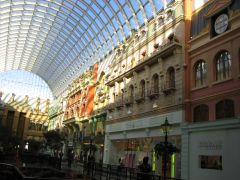
\includegraphics[width=.45\linewidth]{gfx/example_1}} \quad
        \subfloat[Pan ma signo.]
        {\label{fig:example-b}%
         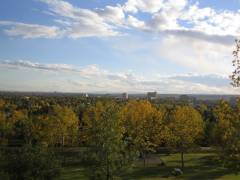
\includegraphics[width=.45\linewidth]{gfx/example_2}} \\
        \subfloat[Methodicamente o uno.]
        {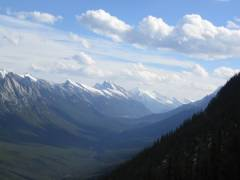
\includegraphics[width=.45\linewidth]{gfx/example_3}} \quad
        \subfloat[Titulo debitas.]
        {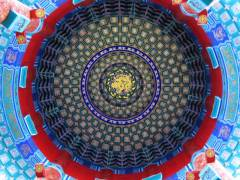
\includegraphics[width=.45\linewidth]{gfx/example_4}}
        \caption[Tu duo titulo debitas latente]{Tu duo titulo debitas
        latente.}\label{fig:example}
\end{figure}


%*****************************************
%*****************************************
%*****************************************
%*****************************************
%*****************************************

%\addtocontents{toc}{\protect\clearpage} % <--- just debug stuff,
%ignore

%\parskip = \baselineskip %??
%\setlength{\parindent}{0pt}

% % ************************************************
\chapter{Introduction}\label{ch:Introduction} 
% ************************************************

Brain network connectivity, the description of links between the
brain's computational units, lies at the heart of many theories trying
to explain the exceptionally diverse and robust functionality of the
brain. As an essential component in the investigation of the emergence
of its unique cognitive abilities, brain connectivity is often
associated with memory and the remarkable performance in various
perception tasks. Connectivity is, in its essence, a purely abstract
concept and therefore intimately tied to mathematical
theories. Heavily relying on a mathematical framework for the analysis
and discussion of network connectivity, this aspect of brain research
is an exciting example and highly relevant example of applied
mathematics.

In the field of theoretical and computational neuroscience neural
network models are studied as of brain networks. Studies interested in
the dynamical aspect for example investigate . The standard model for
such simulations is that of random
graph \parencite{Brunel2000}. However, results over the last years
show that local cortical circuits display highly non-random
connectivity features \parencite{Song2005, Perin2011}. It is unclear
how to incorporate such as underlying remain yet to be identified.
unclear how to incorporate. Important to identify underlying rules.

The search underlying principles has
since \parencite{Klinshov2014}. In an effort to contribute to this
discussion, we here investigate anisotropy in connectivity. Motivated
from observations of stereotypical morphology, the may not only
provide but further can be a first step towards network models. Making
sure that, the hope is not only to contribute but to help network
model.

\section{Overview}\label{sec:all_overview}

Following the introduction and this outline, a short overview of the
biological terms frequently appearing throughout this text is given as
reference at the end of this chapter. The central mathematical objects
in this study, various directed graph models, are then introduced and
discussed in detail in Chapter~\ref{ch:graph_theory}. Building on
these concepts, Chapter~\ref{ch:network_model} introduces the
anisotropic network model as the main object of investigation in this
thesis. Next to an in-depth motivation of the anisotropic connectivity
concept, the chapter also introduces the rewiring of networks and a
measure for anisotropy, laying the groundwork for the analysis of
structural features in anisotropic networks in
Chapter~\ref{ch:structural_aspects}. First investigating standard
network attributes like degree distributions and small-world measures,
analysis of higher order connectivity in the latter part of the
chapter reveals the highly interesting emerging patterns in
anisotropic networks. Closing the structural analysis with a critical
discussion of the obtained results, an outlook in
Chapter~\ref{ch:dynamical_aspects} . 



\section{Biology of Neural Networks}\label{sec:Biology} 



The fundamental computational units in brain networks are
neurons\index{neuron}, electrically excitable cellular elements that
process and transmit information by a cell type dependent regime of
electrical and chemical signals. Neurons are linked through
synapses\index{synapse}, forming together an expansive, interconnected
network of different neuron types, dividing into functionally and
anatomically distinct areas. The number of neurons in the average
human brain is estimated at about 86 billion, connected by
$10^{14}$ - $5\times10^{15}$ synapses \parencite{Herculano2009,
  Drachman2005}. Among the different brain areas studied, the
multilayered cerebral cortex\index{cortex} stands out as a region of
particular interest with many studies analyzing its structural and
dynamical features.

The principal excitatory neuron type in cortical
networks\index{cortical network} are pyramidal cells\index{pyramidal
  cell}. Connection between those neurons are mainly of chemical
nature, in the synaptic contacts between cells the release and
consequent reception of neurotransmitters transmits electrical
signals. While cortical networks are considered sparse, pyramidal
cells typically receive tens of thousands excitatory and several
thousand inhibitory inputs, making up for an overall connectivity of
about $10\%$ in local networks \parencite{Spruston2009}. Such synaptic
contacts are inherently asymmetric; signals travel from the cell body
of a neuron along the axon to be transmitted at a synapse contacting
the dendritic tree of the post-synaptic neuron. Morphology of axon and
dendrite are characteristically different; it is this difference that
is taken up in this study and serves as a basis for the network model introduced in Chapter~\ref{ch:network_model}.

To enable we introduce 
For Brain networks . They are well presented by the mathematical
object of a directed graph, which will be discussed in detail in the
following chapter.









%%% Local Variables: 
%%% mode: latex
%%% TeX-master: "../dplths_document"
%%% End: 

% % ************************************************
\chapter{Biology}\label{ch:Biology} 
% ************************************************




%%% Local Variables: 
%%% mode: latex
%%% TeX-master: "../ClassicThesis"
%%% End: 

% % ************************************************
\chapter{Graph Theory}\label{ch:Graph_theory} 
% ************************************************
In this chapter we review basic graph theory and explain how these
terms are applicable in the context of biological neural networks. We
begin with the definition of directed graphs:

\section{Definitions \& Basics}

References for this chapter:
\url{http://nlab.mathforge.org/nlab/show/graph},
\url{http://nlab.mathforge.org/nlab/show/quiver}, \parencite{Bang-Jensen_Digraphs} 


%  \begin{definition}[Graph, Order] A \textbf{graph} is a pair of sets $G
% =(V,E)$, consisting of the \textbf{vertex set} $V(G)=V$ and the
% \textbf{edge set} $E(G)=E$, such that $E \subseteq V \times V$.  The
% number of vertices of a graph $G$ is its \textbf{order} $|G|$, the
% number of edges is denoted by $||G||$.  A graph of order $0$ or $1$ is
% called \textit{trivial}.
%   \end{definition}

%   The object of interest in my thesis will be directed pseudographs,
% but I will still have to think about how to
%   \begin{itemize}
%   \item call them, graphs, directed graphs, etc..
%   \item think about the weights(!!)
%   \item think about definitions
%   \end{itemize}

%   \bigskip




\begin{definition}[Directed graphs]
  A \textbf{directed pseudograph} $G$ consists of two finite \red{(,
    non-empty?)} sets $V$, the \textit{set of vertices} of $G$, and
  $E$, the \textit{set of edges} of $G$, and two maps
  \[
  s,t: E \to V,
  \]
  the \textit{source} and \textit{target functions} of $G$. A
  \textbf{directed multigraph} is a directed pseudograph without
  \textit{loops}, that is the map $d = (s,t):E \to V^2$ already maps
  maps to $V^2\setminus\Delta_V$, where $V^2 = V \times V$ denotes the
  cartesian product and $\Delta_V = \{(x,x)|x \in V\} \subseteq V^2$
  the diagonal. Similarily, a \textbf{directed loop graph} is a
  directed pseudograph where $d$ is injective. Finally, a
  \textbf{simple directed graph} can be defined as a directed
  pseudograph where $d$ is both injective and already maps to
  $V^2\setminus\Delta_V$.
\end{definition}

Thus, in simple directed graphs, neither parallel edges nor loops -
edges between the same vertex - are allowed, whereas directed
multigraphs and directed loop graphs admit one of them respectively.

\red{Say something about what "directed graph" means here.}

Given a directed graph $G$, we denote with $V(G)$ the set of vertices
of $G$ and call it the \textbf{vertex set} of $G$. Analogously, the
\textbf{edge set} $E(G)$ of $G$ denotes the set of edges of $G$. This
means, for a directed graph specified as $G = (V_G,E_G,s_G,t_G)$, we
have \[V(G) = V_G \quad \mathrm{and} \quad E(G) = E_G.\]


\begin{figure}
  % \includestandalone[width=\textwidth]{gfx/tikz/directed_graph_types}
  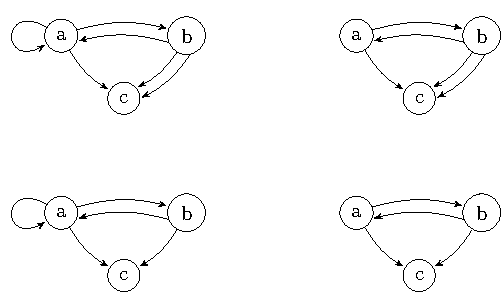
\includegraphics{tikz/directed_graph_types.pdf}
  \caption{From top left to bottom right, typical examples of the
    defined graph types: A) directed pseudograph, B) directed
    multigraph, C) directed loop graph D) simple directed
    graph.} \label{fig:M1}
\end{figure}


A \textbf{morphism} $\phi: G \to H$, between two directed graphs
$G=(V_G,E_G,s_G,t_G)$ and $H=(V_H,E_H,s_H,t_H)$, consists of a pair of
maps $\phi_V: V_G \to V_H$ and $\phi_E: E_G \to E_H$, such that
\[
s_H \circ \phi_E = \phi_V \circ s_G \mathrm{\quad and \quad} t_H \circ
\phi_E = \phi_V \circ t_G,
\]

that is such that the following diagram commutes:

\begin{align*} 
  \xymatrix@+=1.3cm{E_G \ar^{t_G}@<0.66ex>[d] \ar_{s_G}@<-0.66ex>[d]
    \ar^{\phi_E}[r] & E_H \ar^{t_H}@<0.66ex>[d]
    \ar_{s_H}@<-0.66ex>[d]\\ V_G \ar^{\phi_V}[r] & V_H}
\end{align*}

\bigskip

A morphism $\varphi: G \to H$, between two directed pseudographs $G$
and $H$ is an \textbf{isomorphism}, if the maps $\varphi_V: V_G \to
V_H$ and $\varphi_E: E_G \to E_H$ are bijective. Two directed
pseudographs are called \textit{isomorphic} if there exists an
isomorphism inbetween them.

\begin{remark}
  The last definition implies that, if there exists an isomorphism
  $\varphi: G \to H$, an isomorphism $\psi: H \to G$ can be
  found. This isomorphism is, of course, easily constructed via
  $\psi_V: V_H \to V_G, v \mapsto \varphi_V^{-1}(v)$, $\psi_E: E_H \to
  E_G, e \mapsto \varphi_E^{-1}(e)$.
\end{remark}

\begin{definition}[Weighted directed graphs]
  A \textbf{weighted directed graph} is a directed graph $G$ along
  with a mapping $\omega: E(G) \to \mathbb{R}$, called the
  \textit{weight function}. Similarily, a \textbf{vertex-weighted
    directed graph} is a directed graph with a mapping $\nu: V(G) \to
  \mathbb{R}$.
\end{definition}

\begin{remark} \red{(heavy draft)}, title: A directed graph category
for biological neural networks, in a bordered box?\\ Certainly, a
weighted directed pseudograph is the most fitting mathematical
modelling to the biological situation, since self connections and
multiple synapse are not only plausibel (source?) but the
rule. However there is one abstraction we can make by adding together
the synaptic weights - NEST is doing it..\\ Also think about
\textbf{inhibitory, excitatory}. Suggestion: edge weights $\omega:
E(G) \to \mathbb{R}^{+}$ \textbf{and} vertex weights $\nu: V(G) \to
\{-1, 1\}$. Synaptic weight $\mathrm{syn}(e)$ for edge $e$ is
then \[\mathrm{syn}(e) = \nu(s(e))\,\omega(e).\] Benefit: Synapse from
one neuron are either excitatory or inhibitory but not mixed as in
bio.
\end{remark}


\begin{remark}[Equivalent definiton for directed loop graphs]

  A directed loop graph $G$ can be equivalently defined as a pair of
  finite\red{(, non-empty?)} sets $V$, the \textit{set of vertices} of
  $G$, and $E \subseteq V^2$ the \textit{set of edges} of $G$. For an
  edge $(x,y) \in E$, we call $x$ the \textit{source} and $y$ the
  target of the edge $(x,y)$.

  Source and target functions are then uniquely determined as the
  projections on the first and second component, $s = \mathrm{pr}_1, t
  = \mathrm{pr}_2: E(G) \to V.$ Conversely, the edge set $E(G)
  \subseteq V^2$ can be determined from the source and target
  functions as $E:=\{(s(e),t(e)) | e \in E\}$. The trivial identities
  $(x,y) = (\mathrm{pr}_1(x,y),\mathrm{pr}_2(x,y))$ and
  $\mathrm{pr_1}(s(e), t(e)) = s(e)$ with $\mathrm{pr_2}(s(e), t(e)) =
  t(e)$ quickly verify the equivalence of the definitions.

  Given a directed loop graph $G$, we often assume the graph to be
  given in this form and write edges as $e=(x,y)$. Note that this
  concept is more complicated to introduce for directed pseudographs,
  since parallel edges $e$ and $e'$ should to be differentiated in the
  egde set of $G$, establishing the need for $E(G)$ to be a multi- or
  indexed set, notions we are trying to avoid in this document.

\end{remark}




% A given directed loop graph $G = (V,E,s,t)$, can always be
% represented by a canonical isomorphic directed loop graph $G' =
% (V,E')$, where $E':=\{(s(e),t(e)) | e \in E\} \subseteq V^2$. For a
% directed loop graph $G'$ in canonical form, the source and target
% functions $s',t'$ do not need to be specified, since they are uniquely
% determined as the projections on the first and second component, $s' =
% \mathrm{pr}_1, t' = \mathrm{pr}_2$. Wait, not so easy because
% multi-sets, however add synaptic strength of parallel edges to make
% directed loop-graphs! (Bang-Jensen)



From now on any \textit{directed graph} is assumed to be a directed
loop graph. Although most, if not all, concepts work for directed
pseudographs just as well, we want to start to heavily use the
canonical edge representation, which when talking about pseudograps
makes problems as mentioned before.

\begin{remark}[More Notation] 
  \red{- Check, do I really need this?} For a pair of vertex sets $X,Y
  \subseteq V(G)$ of a directed graph $G$ we write
  \[
  (X,Y)_G = \{(x,y) \in E(G) | x \in X, y \in Y \}
  \]
  for the set of edges with source in $X$ and target in $Y$. For
  vertex sets with a single element $X = {x}$, we also write $(x,Y)_G$
  and mean the edges with source $x$ and target in $Y$.
\end{remark}


\begin{remark}[In- and out-degree] 
  For a directed graph $G$ the \textbf{in-degree} $d^-_G(x)$ of a
  vertex $x$ is defined as the number of edges of $G$ with target $x$,
  that is
  \[
  d^-_G(x) = \left|(V(G),x)_G\right|.
  \]
  Similarily, the \textbf{out-degree} $d^+_G(x)$ of $x$ is defined as
  \[
  d^+_G(x) = \left|(x, V(G))_G\right|,
  \]
  the number of edges in $G$ with source $x$.
\end{remark}

\begin{remark}[Side]
  In some literature about directed graphs (Bang-Jensen), loops are
  \textit{not} counting towards the in- or out-degree of vertex. In
  the light of neural network however, we specifically want to count
  loops as well.
\end{remark}

A basic property of the in- and out-degree in directed graphs is that
number of in-degrees of every vertex, as well the sum of every
out-degree, equal the total number of edges:

\begin{proposition}
  In every directed graph $G$, we have
  \[
  \sum_{x \in V(G)} d^-(x) = \sum_{x \in V(G)} d^+(x) = | E(G) |.
  \]
\end{proposition}

\begin{proof}
  Since $(V(G),x)_G \cap (V(G),y)_G = \emptyset$ for $x \ne y$, we can
  write
  \[
  \sum_{x \in V(G)} d^-(x) = \left| \bigcup_{x \in V(G)} (V(G),x)_G
  \right| = \left| (V(G),V(G))_G \right| = | E(G) |.
  \]
  Analogously for the out-degree.
\end{proof}


\subsection*{Walks and distances}

Let $G$ be a directed graph \red{(what does it mean here?)}. A
\textbf{walk} $W$ in $G$ is an alternating sequence
$(x_1,e_1,x_2,e_2,x_3,\ldots,x_{n-1},e_{n-1},x_n)$ of of vertices
$x_i$ and edges $e_i$ from $G$, such that
\[
s(e_i) = x_i \quad \mathrm{and} \quad t(e_i) = x_{i+1}, \:\,
\mathrm{for}\, i=1,..,n-1,
\]
that is, such that the vertices are connected by the edges inbetween
them. We denote the set of vertices $(x_1,\ldots,x_n)$ of $W$ as
$V(W)$ and the sequence of edges $(e_1,\dots,e_{n-1})$ as $E(W)$
\red{(need it?)}.

The vertices $x_1$ and $x_n$ are called the \textit{end vertices} of
$W$ and we also say that $W$ is an $(x,y)$-walk. The \textbf{length}
of $W$ is defined as the length of the sequence of edges; a walk
consisting of only one vertex has length zero. \red{ colon, really?}


\begin{definition}[Distance]
  The \textbf{distance} of two vertices $x$,$y$ in a directed graph
  $G$ \red{(means?)}, is defined as the minimum length of an
  $(x,y)$-walk, if any such walk exists, otherwise
  $\operatorname{dist}(x,y)=\infty$. In short,
  \[
  \operatorname{dist}(x,y) = \inf \{|E(W)| \mid
  W\,\mathrm{is}\,(x,y)\mathrm{-walk}\}.
  \]
  \red{$|E(W)|$ is not explained. Necessary?}
\end{definition}

\begin{proposition}
  The distance function $\operatorname{dist}: V(G) \times V(G) \to
  \mathbb{N}$ of a directed graph $G$ satisfies the triangle equality,
  \[
  \operatorname{dist}(x,z) \le \operatorname{dist}(x,y) +
  \operatorname{dist}(y,z), \:\: \mathrm{for}\:\, x,y,z \in V(G).
  \]
\end{proposition}

\begin{proof}
  Let $x,y,z$ be vertices in $G$. If either no $(x,y)$-walk or
  $(y,z)$-walk exists, the inequality holds by definition. Other wise,
  let $W$ be an $(x,y)$-walk of minimal length and let $U$ be a
  $(y,z)$-walk of minimal length. Certainly, by concatenating $W$ and
  $U$ we obtain an $(x,z)$-walk of length $|E(W)| + |E(U)| =
  \operatorname{dist}(x,y) + \operatorname{dist}(y,z)$, proofing
  that \[ \operatorname{dist}(x,z) \le \operatorname{dist}(x,y) +
  \operatorname{dist}(y,z).
  \]
\end{proof}





%   \begin{definition}[Neighbour, adjacent] Two \textbf{vertices} $x,y \in
% V(G)$ of $G$ are called \textit{adjacent} or \textit{neighbours} if
% there is an edge between $x$ and $y$, $(x,y) \in E(G)$. Two
% \textbf{edges} $e \neq f$ are \textit{adjacent} if they have an end in
% common.
%   \end{definition}


More to do:

\begin{itemize}
\item summarize category of directed (weighted) pseudographs
\item weights!
\item vertices will also be called nodes and neurons, edges will also
  be connections or synapses.
\item subgraphs
\item vertex set, edge set $E(G), V(G)$.
\item $\omega(e)$ is weight, connection strength or synaptic weight
  (as a side remark
\item extend to category of weighted directed pseudographs
  (isomorphisms)
\item path
\item adjacency matrix
\item converses of graph related to opposite category?
\item in- and out-degree
\item triangle inequality for distance, $\mathrm{dist}(x,z) \leq
  \mathrm{dist}(x,y) + \mathrm{dist}(y,z)$
\end{itemize}

\bigskip

\section{Random Graph Theory}

For this chapter, as it is common and practical when talking about
random graphs, we move away from the the abstract notion of graphs and
their equivalence classes and consider \textit{labeled graphs}, where
the edge set of a graph with $n$ vertices takes the form $V =
\{1,\ldots,n\}$.




\subsection{Erd\H{o}s-R\'{e}nyi graphs}

References: Newman, Erdos1960, Erdos1959, Gilbert1959, 
Wikipedia, \parencite{West_Graph-theory}
		
		
\begin{definition}[Terms used]
  Graphs with $n$ vertices: $G^n = \{G| G\,\mathrm{is\,
    graph\,(means??)},\, |V(G)| = n\}$
\end{definition}
		
\begin{remark}[Expected number of edges in a directed Erd\H{o}s-R\'{e}nyi graph (DERG)]
  $X: G^n \to \mathbb{R}, G \to |E(G)|$, discrete random variable,
  with probability distribution $G(n,p) =\operatorname{B}(n^2,p)$,
  binomial distribution. That is, distribution of $X$ via probability
  mass function $P(X=k) = {{n^2} \choose k} p^k\,(1-p)^{n^2-k}$. Thus
  $\operatorname{E}(X)$ equals expect edges in DERG. We have of
  course, since $G(n,p)$ binomial,
  \[
  \operatorname{E}(X) = pn^2. \mathrm{\:(if\,self-edges!)}
  \]
  Then, of course, the \textbf{mean in-}  and \textbf{out-degree} is \[ \langle
  d^{\mathrm{in}} \rangle = \langle d^{\mathrm{out}} \rangle =
  \frac{\langle |E(G)| \rangle}{|V(G)|} = np.\] \textit{Does this make
    sense? Define everything properly!!}
\end{remark}

\subsection{Random Graph Model - Gilbert}\label{sec:gilbert_graph}



% From Graph clustering - Satu Elisa Schaeffer - 2007
% 
% [84] P. Erdos, A. Rényi, On random graphs I, in: Selected Papers
% of Alfréd Rényi, vol. 2, Akadémiai Kiadó, Budapest, Hungary,
% 1976, pp. 308–315. First publication in Publ. Math. Debrecen
% 1959.
% [85] P. Erdos, A. Rényi, On the evolution of random graphs,
% in: Selected Papers of Alfréd Rényi, vol. 2, Akadémiai Kiadó,
% Budapest, Hungary, 1976, pp. 482–525. First publication in
% MTA Mat. Kut. Int. Közl. 1960.





%%% Local Variables: 
%%% mode: latex
%%% TeX-master: "../dplths_document"
%%% End: 

 % ************************************************
\chapter{Network Model}\label{ch:Network Model} 
% ************************************************

Referring to anisotropic characteristics in local cortical circuits of
the rat's brain, a network model implementing anisotropic tissue
geometry is developed. The introduction of a rewiring algorithm and
qualitative anisotropy measure %quantitative ??
lay the foundation for the analysis of structural aspects of this
model in Chapter~\ref{ch:structural_aspects}.

%\section{Introduction}\label{sec:intro_model}
\clearpage
\section{Anisotropy in Neural Connectivity}\label{sec:biol_anisotropy}

Neurogeometry\index{neuro geometry} addresses the problem of inferring
synaptic connectivity from the geometric shapes of axon and
dendrites. A fundamental concept in this field is that of a
\textit{potential synapse}\index{potential synapse}
\parencite{Stepanyants2002}. Defined as the potential axonal-dendritic
connection of two neurons, present whenever the axon of one neuron is
within a spatial distance $s$ of the dendrite of the other, it is a
necessary, although not sufficient, condition for the formation of a
synaptic connection (\autoref{fig:potential_synapse}). The existence
of such close appositions solely depends on dendritic and axonal
anatomy; identification of defining morphological characteristics in
both axon and dendrite would therefore allow for a model of local
network connectivity, assuming for example that a certain ratio $r$ of
potential synapses turn into active contacts independently. It is the
hope that such a model, motivated from the geometry of a neuron's
functional compartments, not only displays inherent patterns of
connectivity similar to what has been observed in biological networks,
but also proofs itself as a testing ground for how this connectivity
may affect network dynamics.

\vspace{-0.21cm}
\definecolor{lightgray}{rgb}{0.88, 0.88, 0.88}
\begin{center}
 \setlength{\fboxrule}{0pt}
 \fcolorbox{black}{lightgray}{
   \begin{minipage}[c]{0.90\textwidth}

     \vspace{0.1cm}
     \setlength{\intextsep}{0pt}%
     \setlength{\columnsep}{8pt}%
     \begin{wrapfigure}{r}{0.65\textwidth}
       \captionsetup{labelformat=empty,labelsep=none}
       \centering
       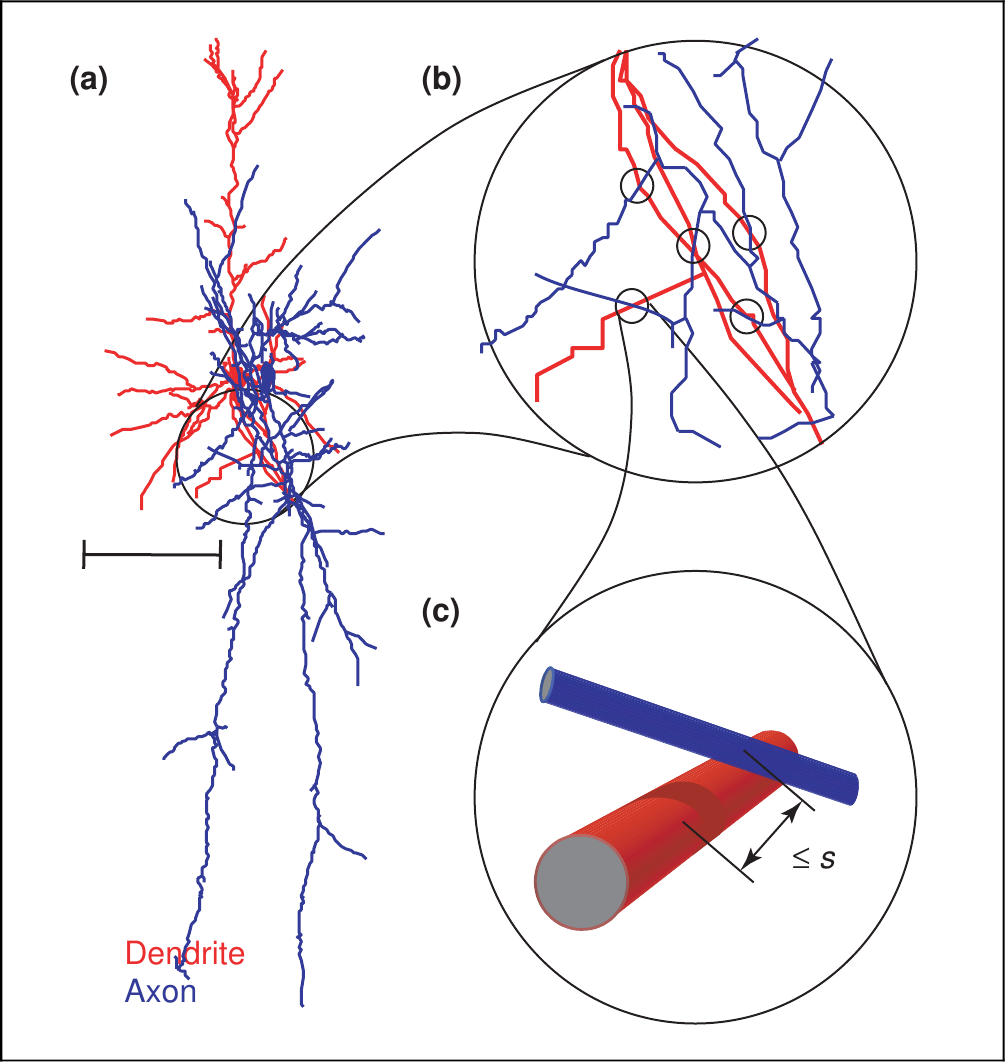
\includegraphics[width=\linewidth]{img/potential_synapse2.png}
       \vspace{-35pt}
       \caption{}
       \label{fig:potential_synapse}
     \end{wrapfigure}

     \footnotesize \textbf{Potential Synapse} 
     \smallskip

     Close ap\-positions be\-tween den\-drite and axon
     are a necessary condition for the formation of a synapse. \textbf{(a)}
     3-D reconstructions of a py\-ra\-mi\-dal cell den\-drite in red, axon of a
     regular spiking non-pyramidal cell in blue. \textbf{(b)-(c)}
     Overlapping arbors allow for several potential synapses whenever
     dendrite and axon are within a spatial distance $\leq s$. Values for
     $s$ depend on the type of synapse, typically between
     0.4-\SI{2}{\micro\meter}. Scale bar: \SI{100}{\micro\meter},
     \SI{30}{\micro\meter}, \SI{3}{\micro\meter} in (a),(b),(c)
     respectively. Image from \textcite{Stepanyants2005}. \hfill \textbf{4.1}

     \vspace{0.1cm}
   \end{minipage}}
\end{center}
%\vspace{-0.12cm}


Finding stereotypical anatomical characteristics however is difficult,
as axonal morphology is, in general, highly diverse
%------------------------------------------------
\marginpar{high variability in axonal morphology} 
%------------------------------------------------ 
\parencite{Debanne2004}. Across different species,
distinct regions in the central nervous system and different neuron
types, axons display a wide variety of shapes characterized by
morphometric parameters such as total length, branching complexity and
axonal extent \parencite{Ropireddy2011}. Typical examples of distinct
morphology include the T-shaped axons of cerebellar granule cells
branching only at a singular point \parencite{Cajal1911}, and axons of hippocampal CA3
pyramidal cells, which, in stark contrast, may feature up to 40
branches resulting in a total length of axon collaterals of up to
\SI{12}{\milli\meter} \parencite{Ishizuka1990}.

It is therefore imperative to confine this analysis to a specific
brain region and neuron type. In this study, we set the focus on
circuits of pyramidal cells in the mammalian cortex.
%?? Cortex does this
%?? Cortex is this well studied
%?? Here we go
More specifically, local circuits of thick tufted layer V
pyramidal neurons in the rat's somatsosensory cortex have been the
target of advanced
experimentation \parencite{Song2005,Perin2011,Romand2011, Ramaswamy2012}, and will
serve as a benchmark for results in neural morphology and network
connectivity in this report.


\begin{figure}[!htbp]
  \centering 
  \makebox[0.875\textwidth]{%
    \begin{overpic}[width=0.4\textwidth]{%
        img/network_model/p14rr_1.pdf}
      \put(3,92){\small\textbf{A}}
    \end{overpic}
    \hfill
    \begin{overpic}[width=0.4\textwidth]{%
        img/network_model/p14rr_1_axon_traced_soma.pdf}
      \put(3,92){\small\textbf{B}}
    \end{overpic}
    }%
  \caption{\textbf{Tracing axonal branching of a pyramidal cell} In a
    3-D model reconstructed from biocytin-labeled thick-tufted layer V
    pyramidal cells in the somatosensory cortex of postnatal (day 14)
    Wistar rats, \textcite{Romand2011} depict dendritic compartments in
    red, axonal compartments in blue.  \textbf{A)} A
    \SI{600}{\micro\meter} window centered on the soma of the pyramidal
    cell shows the main stem of the cell's axon projecting downwards in a
    straight line, collaterals branching at various angles. \textbf{B)}
    Using image manipulation software, axon morphology was manually traced
    and is emphasized in black.}    
  \label{fig:romand_axon_trace}
\end{figure}


Axonal morphology of pyramidal cells in the cerebral cortex is well
described. From the soma the single main stem of the axon
%------------------------------------------------
\marginpar{cortical axons form straight lines, arborize profusely} 
%------------------------------------------------ 
originates and projects downwards, describing a trajectory closely
resembling a straight line \parencite{Braitenberg_Cortex}. At
arbitrary points along this path, collaterals branch off at various
angles and constitute themself linear paths until they further ramify
or terminate. Displaying a high degree of ramification, axonal trees
of cortical pyramidal cells build, in general, complex
structures \parencite{Petersen2003,Ramaswamy2012}. Cortical slice
experiments analyzing neural anatomy are typically constrained by a
slice thickness of \SI{300}{\micro\meter}. On this scale, 3-D
reconstruction from labeled thick tufted layer V pyramidal cells
reveals characteristic morphology of the axonal tree
(\autoref{fig:romand_axon_trace}). The downwards projecting, straight
axon branches at several points, forming collateral branches that
travel in linear path as well.

In a statistical view, this characteristic axonal morphology results
in high axon branch densities along the main stem, whereas distant
regions display a relatively low density
(\autoref{fig:axon_heat}). Specifically, axon collaterals do not
cluster around the soma but align with the main stem's projection. As
presence of an axonal branch constitutes a necessary condition for a
potential synapse, a higher concentration of potential and,
subsequently, realized synapses is expected in regions of high branch
density. For a coherent picture of local connectivity profiles,
however, dendritic morphology needs to be considered as well. 

 
\begin{figure}[!htbp]
  \centering 
  \makebox[0.875\textwidth]{%
    \begin{overpic}[width=0.4\textwidth]{img/network_model/p14rr_1_trace_soma.pdf}
      \put(3,92){\small\textbf{A}}
    \end{overpic}
    \hfill
    \begin{overpic}[width=0.4\textwidth]{img/network_model/axon_heat_correct_soma.png}
      \put(3,92){\small\textbf{\textcolor{white}{B}}}
    \end{overpic}
    }%
    \caption{%
      \textbf{Illustrating axonal branch density}
      In a sample of 5 reconstructions from thick-tufted layer V pyramidal
      cells \parencite{Romand2011}, tracing axonal morphology illustrates
      characteristic branch density along the axon's main
      stem. \textbf{A)} Example of extracted axonal tree. Outline manually
      traced using image manipulation software. Soma indicated by
      triangle. Original data from \textcite{Romand2011}. \textbf{B)}
      Overlaying 5 axonal trees extracted as in A), 
      % ?? show Appendix?  Sumatra label?? colorbar??
      applying a Gaussian filter and displaying high axon densities in
      warm colors, illustrates the characteristic higher branch
      densities along the axon's main stem.}
  \label{fig:axon_heat}
\end{figure}


Dendritic anatomy of cortical pyramidal cells is inherently bipartite.
From the soma several \textit{basal dendrites}\index{basal dendrite}
emerge and extend into arbitrary directions, branching profusely until
they terminate . The single \textit{apical dendrite}\index{apical
  dendrite} emerges from the apex of the pyramidal cell and ascends in
a linear trajectory, forming occasional collateral branches until
finally terminating into the apical tuft, where the dendrite branches
several times to form a tree like structure \parencite{Feldman1984}.
%------------------------------------------------
\marginpar{basal dendrites dominate local connectivity} 
%------------------------------------------------  
On the scale of typical cortical slice thickness, however, the apical
dendrite is cut off and the basal dendrite dominates the dendritic
morphology and potential of dendritic-axonal connections
(\autoref{fig:dendrite_heat}). The radial extension of dendritic
branches results in a high concentration of dendritic branches around the
soma, much in the contrast to the findings of axonal branch densities
before.

\begin{figure}[!ht]
  \makebox[0.875\textwidth]{%
    \begin{overpic}[width=0.4\textwidth]{%
        img/network_model/p14rr_1.pdf}
      \put(3,92){\small\textbf{A}}
    \end{overpic}
    \hfill
   \begin{overpic}[width=0.4\textwidth]{img/network_model/p14rr_1_traced_soma.pdf}
      \put(3,92){\small\textbf{B}}
    \end{overpic}
    }
  \vfill
  \vspace{0.3cm}
  \makebox[0.875\textwidth]{%
    \begin{overpic}[width=0.4\textwidth]{img/network_model/p14rr_1_dendrite_trace_scale.pdf}
      \put(3,92){\small\textbf{C}}
    \end{overpic}
    \hfill
    \begin{overpic}[width=0.4\textwidth]{img/network_model/dendrite_heat_correct_soma.png}
      \put(3,92){\small\textbf{\textcolor{white}{D}}}
    \end{overpic}
    }%
  \caption{\textbf{Dendritic morphology and branch density}
    Using neuronal morphology of thick-tufted layer V
    pyramidal cells recorded by \textcite{Romand2011}, dendritic
    anatomy is traced and combined to illustrate high
    branch density around the soma. \textbf{A)} In a
    \SI{600}{\micro\meter} window centered on the soma, basal
    dendrites (red) are visible extending around the soma. The ascending
    thick apical dendrite (red) is cut off and apical tuft is not
    shown. \textbf{B)-C)} Manual tracing of dendritic outlines
    in five samples (one shown), allows for clearer identification of
    stereotypical morphology and later analysis. \textbf{D)} Combining
    5 dendritic outlines as shown in C) and subsequent Gaussian
    filtering reveals the relatively high dendritic branch density
    around the soma.
  }%?? sumatra label
  \label{fig:dendrite_heat}
\end{figure}


Combining the above results of dendritic and axonal branch densities
in the light of neurogeometry, a clear concept of anisotropy of neural
connectivity emerges. As dendritic branches of potential post-synaptic
targets extend radially from the soma and do not display a preferred
direction, target neurons for outgoing synaptic contacts originating
from a single pyramidal cell, cluster around the downwards projecting
axon (\autoref{fig:neural_anisotropy}). %?? high branch density
                                %correlates directly with expected
                                %number of contacts!
\begin{figure}[!ht]
  \centering 
  \makebox[0.875\textwidth]{%
    \begin{overpic}[width=0.4\textwidth,frame]{img/network_model/axon_dendrite_meet.pdf}
      \put(3,92){\small\textbf{A}}
    \end{overpic}
    \hfill
    \begin{overpic}[width=0.4\textwidth,frame]{img/network_model/axon_dendrite_meet_schema_dense.pdf}
      \put(3,92){\small\textbf{B}}
    \end{overpic}
    }%

    \caption{%
      \textbf{Connected neurons of a single pyramidal cell align with
        axonal projection} Reducing the full axonal (blue,
      cf. \autoref{fig:romand_axon_trace}) and dendritic trees (red, gray,
      cf. \autoref{fig:dendrite_heat}) as shown for two neurons in A)
      to their stereotypical axonal (blue) and dendritic profiles
      (red, gray) in B), demonstrates how connected neurons (red) tend
      to cluster around the pre-synaptic axon's profile, as spatial
      closeness constitutes a necessary condition for the formation of
      contacts. Unconnected neurons (gray) are found distant from the
      axon's projection, but not necessarily distant from the soma. }
  \label{fig:neural_anisotropy}
\end{figure}
%\vspace{-0.2cm} 
% Why is anisotropy so good??
% It becomes apparent that
% connected neurons are located along the main axon in much higher
% concentration than in directions that diverge from the axon's
% projection. 
In their in-depth study, \textcite{Stepanyants2005} confirm the
overrepresentation of potential synapses along the axon for pyramidal
cells. Consistent with the notion that stereotypical morphology of
pyramidal cells is intrinsic to the local network's connectivity
profile, they also find that anisotropy of this degree is \textit{not}
present in spiny stellate neurons located in lower-layer-4.



% It is worth noting that this result of anisotropic connectivity does,
% in general, not hold for other brain regions and neurons type. While
% the ad hoc approach taken here is confirmed by an in-depth study of
% \textcite{Stepanyants2005} for cortical pyramidal cells, spiny
% stellate neurons located in lower-layer-4 do not show a clear
% preferred direction for potential synapse.


% Thick tufted pyramidal cells in the rat's somatosensory cortex 

% Owing to this diversity, it is impossible to and it
% is our intent to focus on a specific neuron type and brain region.

% Neuron morphology as well as network connectivity in the rat's
% somatosensory cortex has been thoroughly studied. Even more
% specifically, thick tufted layer V have been the target of studies. 
% \marginpar{focus on TTL5 neurons}


% Neuron morphology and connectivity in the rat's somatosensory cortex
% has been thoroughly studied. As s. 




% the respective axonal
% trees where traced using image manipulation o 

% , showing an apparent anisotropy in neural connectivity, aligning with
% the growth direction of axon's main stem (\autoref{fig:axon_heat}).


% Combing the heatmaps, we obtain clear evidence for anisotropy. In the
% next section we will combine dendritic and axonal morphological
% characteristics into an abstracted geometric model. 

% Identifying anisotropy in neural connectivity as an interesting . In
% this thesis 
% In this study is more specifically focusing in pyramidal neurons in 





\section{Anisotropic geometric graph model}\label{sec:anisotropic_network_model}

% Model tries to be geometric and simple. We therefore

% and propose the following model: along the main stem of the axon in
% constant width. \marginpar{Variable

% width later!}%?? When?


% Implementing the concept of anisotropy in neuronal connectivity
% developed in the last section in a model, we're faced with
% challenges. 

% A first approach. The approach taken here tries to, making anisotropy
% a salient feature in an otherwise standard model. 

In this section we formulate a model of network connectivity
incorporating anisotropy as outlined in the last section. A 

With this in mind, we propose the following model: On a square surface
of side length $e$, a number of $N$ point neurons are randomly,
uniformly distributed.  Connected neighbors are then calculated for
each neuron separately and independently, by determining the randomly,
uniformly distributed direction of the neuron's axon. In this
direction the axon traverses over the surface describing a straight
path, terminating only when an edge of the surface is
reached. Directed contacts are made with every neuron that is within a
width $w(x)$ of the axon's trajectory, where in general $w$ depends on
the axon length $x$ at this point
(\autoref{fig:anisotropic_network_model}).

\begin{figure}[!htbp]
  \centering 
  \makebox{%
    \begin{overpic}[width=0.325\textwidth,frame]{%
        img/network_model/model_dendrite_w.pdf}
      \put(3,91){\small\textbf{A}}
    \end{overpic}
    \hfill
    \begin{overpic}[width=0.325\textwidth,frame]{%
        img/network_model/model_axon_w.pdf}
      \put(3,91){%
        \fboxsep=0pt\colorbox{white}{\small\textbf{B}}
        }
    \end{overpic}
    \hfill
    \begin{overpic}[width=0.325\textwidth,frame]{%
        img/network_model/connectivity.pdf}
      \put(3,91){\small\textbf{C}}
    \end{overpic}
    }%
    \caption{%
      \textbf{Anisotropic geometric network model and interpretations
        of width parameter $\boldsymbol w$} Illustrating the process of
      finding connections for one neuron (large triangle, black), the
      axon describes a linear trajectory in an arbitrary direction and
      until terminating on the surface's edge. Target neurons (red)
      are encountered along the path within a distance $w$, which is in
      \textbf{A)} interpreted as a dendritic radius or, equivalently,
      in \textbf{B)} as a \enquote{bandwith} of the axon. Connections
      to the encountered targets are then established as projections
      in \textbf{C)}, consistent with the directed nature of synapses
      in biological networks (cf. Chapter~\ref{ch:Biology}).}
  \label{fig:anisotropic_network_model}
\end{figure}


The implementation of arbitrary axonal orientation is crucial to the
model. Although cortical axons are described as consistently
projecting downwards \parencite[%
cf. Section~\ref{sec:biol_anisotropy}]{Braitenberg_Cortex}, combining
exclusively vertically aligned axons with the simplified axonal and
dendritic morphological profiles would result in a \enquote{vertically
  staggered connectivity} - neurons could then only project to targets
located below them.  It is in fact not a vertical alignment of axon
orientation, but the anisotropy in neural connectivity - the
observation of neuronal targets aligning with the axonal projection -
that this model tries to capture. 

We will commonly refer to the model defined above as the
\textit{anisotropic geometric network model}. The resulting object of
a realization of the model is a directed graph. More formally we
define realizations as:

\begin{definition}[Anisotropic geometric graph] 
Let $n \in \mathbb{N}$ and $e,w \in (0,\infty)$. An
\textit{anisotropic geometric graph} $G(n,e,w)$ then consists of a
tuple $(G,p,a)$, of a simple directed graph $G$ with $|V(G)|=n$ and
maps \[p:V(G)\to[0,e)^2, \quad a:V(G)\to[0,2\pi),\] such that for every
vertex pair $v,w \in V(G)$ and edge $e\in E(G)$ with $s(e)=v$ and
$t(e)=w$ exists if and only if $\le w$. %what is \le w??
\end{definition}

% \begin{definition}[anisotropic geometric random graph] A anisotropic
%   geometric graph $G(n,e,w)$ is a ran
% \end{definition}

The subsequent is a study of anisotropic geometric graphs. To enable
this analysis, some prior work which composes the rest of this
chapter. Integral to is a numerical implementation. The anisotropic
network model is 





\section{Numerical Implementation}\label{numerical_implementation}

for numerical considerations was achieved in Python. Using convenient 



$N$ Normal distribution. $E$. For a in $N$ 

Computational implementation was achieved by 




Implementing the model as an algorithm in Python, we obtain .

 in connectivity stored in graph
tool \parencite{graph_tool} %?? Fix Display 

Harnessing the computational implementation, we generated a sample of
25 networks with following parameters. 


% \cite{Thomson2002} Axons are not looking for their targets but
% dendrites might, further evidence to focus on axon geometry.

To harness the numerical implemenation to generate networks, a set
of parameters needs to be chosen. The network size $N$ is solely
%------------------------------------------------
\marginpar{determine parameter set to generate sample graphs}
%------------------------------------------------ 
governing computational efforts in subsequent calculations and has
thus been set as $N = 1000$. As shown in ??, only the quotient of
the side length parameter $e$ and axon width $w$  . As such, side
length $e$ is arbitrarily set as $e = 100$ and leaves axon width for
determination. 

First, we determine $w$ to be constant. Although simplistic profiles
(\autoref{fig:axon_heat}) and makes for characteristic distance
distribution as we will see later
(\autoref{fig:distance_theory_compare}), more in line with idea of
abstractness and simplisticity.For small $w$ then, the overall
connection probability $p$ can be approximated as
\[
p = \frac{L w}{E^2},
\]
where $L$ is the average length of the axon until it terminates on a
surface edge. 

\begin{proposition}
Average L
\end{proposition}

\begin{proof}
Hello
\end{proof}

Having established the connection between , 


The final parameter is then the axon-profile width $w$. In their
analysis of connectivity of thick-tufted layer V pyramidal cells in
neonatal rats (day 14), \textcite{Song2005} report an overall connection
probability of $p=0.116$, consistent with prior reports of a cortical
connection probability of $p \approx 0.1$. %?? Which reports?  

\begin{figure}[!htbp]
  \centering
  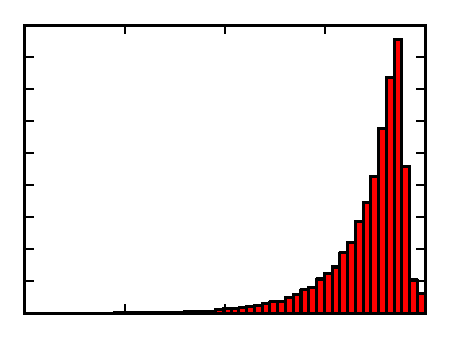
\includegraphics[width=0.8\linewidth]{%
    /users/hoffmann/research/data/axon_width_computation/foo.pdf}%??
  %\includegraphics[width=0.7\linewidth]{plots/test.pdf}
  \caption{\textbf{Tracing axonal branching of a pyramidal cell} In a
    3-D model reconstructed from biocytin-labeled thick-tufted layer V
    pyramidal cells in the somatosensory cortex of postnatal (day 14)
    Wistar rats, \textcite{Romand2011} depict dendritic compartments in
    red, axonal compartments in blue.  \textbf{A)} A
    \SI{600}{\micro\meter} window centered on the soma of the pyramidal
    cell shows the main stem of the cell's axon projecting downwards in a
    straight line, collaterals branching at various angles. \textbf{B)}
    Using image manipulation software, axon morphology was manually traced
    and is emphasized in black.} %??
  \label{fig:determine_axon_width}%??
\end{figure}


Having no further evidence at the time on how to select axon width, we
set $w(x)$ to be constant. This leaves 



With this parameter set we generate a sample of 25 graphs %?? Sumatra:
                                %"N1000w_ax126-flat_graph0-24"






\clearpage
\newpage
\section{Distance dependent connectivity}\label{sec:distance_connectivity}

In Gilbert's random graph model $G(n,p)$, 
\marginpar{Random Graph  Model section~\ref{sec:gilbert_graph}} %?? TITLE
probability of connection $p$ is independently chosen and a fixed
value for all vertex pairs. The anisotropic geometric graph model
introduced in the last %(true??)
section is itself a random graph model - node positions as well as
preferred directions of connection are randomly, uniformly
distributed. In contrast to Gilbert's model however, neither is the
probability of connection between a given vertex pair independent of
the realization of other edges in the graph, nor is it a fixed value -
probabilities strongly depend on internode distance in the
anisotropic geometric graph model introduced.

Analyzing dependencies in the anisotropic model, specifically by
identifying prevalent patterns of connectivity and relating these
modes of non-randomness to biological findings, is the main focus of
Chapter~\ref{ch:structural_aspects}. However, such structural
correlations may not necessarily be an inherent feature of the
network's anisotropy - distance dependent connectivity alone, as
imposed by the model's specific geometry, may be the cause for
emerging dependencies. It is therefore a crucial initial task to map
the anisotropic model's distance dependent connection
probability. Inferring connection probability as a function of
internode distance and comparing it with computational results, in
this section we explore distance connectivity of the anisotropic
network model, securing a vital component in the analysis of
structural features.

Consider a graph $G$. In Gilbert's random graph model the probability
$p$ for a edge between nodes $v,w \in V(G)$ to be realized is a fixed
value; in a geometric graph it is more generally a function of the
distance between the nodes, $d(v,w)$. In short, we write $p(x)$ to
denote the probability that a vertex pair of distance $x$ is
connected,
\[
  p(x) := P\left[(v,w)|\,d(v,w)=x\right].
\]
Owning to the abstract geometric model we defined, this connection
probability is easily computed.

\begin{proposition} \label{distance_prof}
In the anisotropic geometric graph model distance depend connection
probabilities are computed as 
\[
p(x) = \begin{cases} 0.5 & \mathrm{for} \,\, x\le w/2 \\
                       \frac{1}{\pi}
                       \operatorname{arcsin}(\frac{x}{2w}) &
                       \mathrm{for} \,\, x >
                       w/2. \end{cases}
\]
\end{proposition} 

\begin{proof}
  To see this, consider a given source vertex $v$ at $(0,0)$ and a
  possible target $w$, such that $d(v,w) = x$. We may then express the
  target coordinates as $x e^{i\varphi}$, $0 \le \varphi < 2\pi$.

  Figure~\ref{fig:geomtr_prb} illustrates for which angles
  $\varphi$ the node $w$ becomes a valid target for an edge from
  $v$. This intervall

  \begin{figure}[h] 
    \centering 
    \makebox[0.85\textwidth]{%
      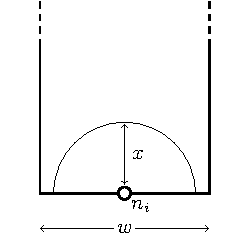
\includegraphics[width=0.4\textwidth]{tikz/geomtr_prb_05.pdf}%
      \hfill
      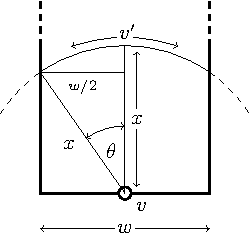
\includegraphics[width=0.4\textwidth]{tikz/geomtr_prb.pdf}% 
    }%
    %\caption{}%??
    \label{fig:geomtr_prb}
  \end{figure}

  For a general $v$ make coordinate transformation

\end{proof}

We can verify this result by computationally extracting the distance
dependencies in the sample graphs generated. 

\begin{figure}[!htbp]
  \centering
  \includegraphics[width=0.8\linewidth]{%
    /users/hoffmann/research/data/sample_graph_analysis/distance_profiles/original/test.pdf} %??
  \caption{\textbf{Predicted distance-dependent connection probability
    profile is matched by numerical computation} In a
    3-D model reconstructed from biocytin-labeled thick-tufted layer V
    pyramidal cells in the somatosensory cortex of postnatal (day 14)
    Wistar rats, \textcite{Romand2011} depict dendritic compartments in
    red, axonal compartments in blue.  \textbf{A)} A
    \SI{600}{\micro\meter} window centered on the soma of the pyramidal
    cell shows the main stem of the cell's axon projecting downwards in a
    straight line, collaterals branching at various angles. \textbf{B)}
    Using image manipulation software, axon morphology was manually traced
    and is emphasized in black.} %??
  \label{fig:distance_theory_compare}%??
\end{figure}





\section{Rewiring}

% In the network configuration introduced in
% section~\ref{sec:network_model} strong directional anisotropy is
% present: Edges originating from one node \enquote{point in the same
%   direction}, that is they connect to other nodes which cluster around
% a. In this section we introduce an algorithm

It is in our highest interest to compare results to. 
%------------------------------------------------
\marginpar{eliminate anisotropy through rewiring}
%------------------------------------------------ 
To this end we introduce an algorithm that preserves
distance-dependent connectivity as found in
Proposition~\ref{distance_prof}, but eliminates anisotropy in network
connectivity by consecutively rewiring existing connections to new
suitable targets.


\begin{algorithm}
Let $N(n,e,w) = (G,P,a)$ be  Then 
\normalfont
\begin{algorithmic}%[1] <-- gives line numbers
\For {$v \in V(N_G)$}
  \For {$e \in E_{\textrm{out}}(v)$}
     \State $x \gets \norm{N_P(v)-t(e)}$
     \State $T \gets \{w \in V(N_G) \mid  x-\varepsilon \leq
     \norm{N_P(v)-N_P(w)} < x+\varepsilon\}$
     \State $t(e) \gets \textrm{choice} T$
  \EndFor
\EndFor

\end{algorithmic}
is defined.
\end{algorithm}

\begin{proposition}
Preserves distance-connectivity.
\end{proposition}

% for every neuron:
%    for every outgoing connection:
%        x = distance to target
%        new_targets = all nodes in distance $(x-\epsilon,x+\epsilon)$


for $\in V(G)$ do 


\vspace{0.5cm}
\begin{figure}[!htbp]
  \centering 
  \makebox[0.85\textwidth]{%
    %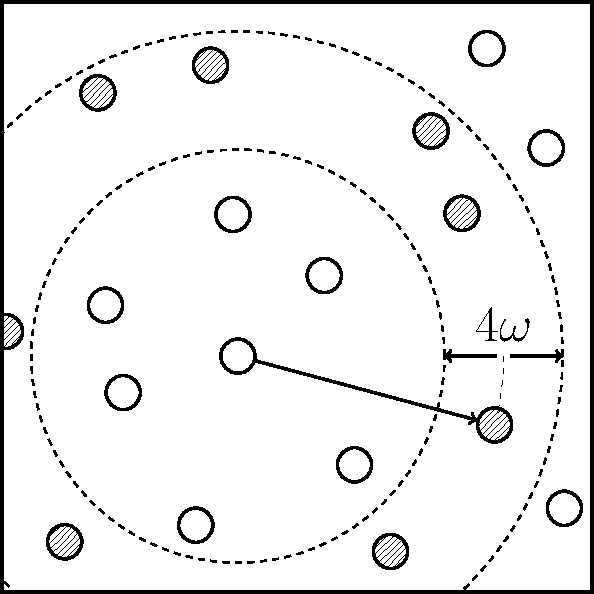
\includegraphics[width=0.4\textwidth]{dist_rew_org.pdf}%
    \begin{overpic}[width=0.4\textwidth, frame]{%
        tikz/distance_rewire_L3.pdf}
      \put(3,105){\small\textbf{Before}}
    \end{overpic}
    \hfill
    \begin{overpic}[width=0.4\textwidth, frame]{%
        tikz/distance_rewire_L4.pdf}
      \put(3,105){\small\textbf{After}}
    \end{overpic} 
  }%
  \caption{\textbf{Rewiring} finding new target in distance $x'$ such
    that $x-\varepsilon \leq x' < x+\varepsilon$.}%??
  \label{fig:distance_rewiring}
\end{figure}

 

\section{Anisotropy Measure}




\section{Summary and Discussion}













%%% Local Variables: 
%%% mode: latex
%%% TeX-master: "../dplths_document"
%%% End: 

% %************************************************
\chapter{Structural Aspects}\label{ch:structural_aspects}
%************************************************

Subjecting the anisotropic network model to a critical
examination of its structural features, we identify prevalent
patterns of connectivity and relate theoretical and computational
results to findings from experiments in the rat's visual cortex.


% 
\section{Introduction}

Investigation \marginpar{
  \begin{center}
    
\includegraphics[width=0.9\linewidth]{img/HCP_text_logo.png}
  \end{center} \vspace{-0.3cm}
  \mbox{\textrm{\href{http://www.humanconnectome.org/}{humanconnectome.org}}}}
of the brain's connectivity is an ongoing endeavour.  Concurrent
collaborative efforts like the Human Connectome Project, the Open
Connectome Project and the Allen Brain Atlas, intent on mapping the
'wiring' of the brain, as well as the continued development of
experimental techniques and computational resources, demonstrate
\marginpar{Open Connectome Project
  \href{http://www.openconnectomeproject.org/}{openconnectomeproject.org}}the
great interest in advancing this field.

Research in brain connectivity spreads over the whole scale
% ---------------------------------------
\marginpar{%
  \begin{center}
    
\includegraphics[width=1.\linewidth]{%
      img/AllenBrainLogo.png}
  \end{center}\vspace{-0.3cm}%
  \mbox{\textrm{\href{http://www.brain-map.org/}{brain-map.org}}}%
  }
% ---------------------------------------
of the brain; from the mapping of fiber pathways between brain regions
at the macroscopic level, to the synaptic connections of individual
neurons on the microscale, researchers are trying to identify the
links that enable the brain its characteristic cognitive abilities.
%Macroscale: Can cite Sporns2004 In the search for structural
connections, these links are of anatomical nature. However,
statistical dependencies and causal relationships between the distinct
computational units in the brain are being researched with equal
emphasis \parencite{Scholarpedia-BrainConnectivity}. Connectivity in
the context of the anisotropic network model introduced in
Section~\ref{sec:anisotropic_network_model}, refers in this chapter to
structural links. So far, we have only briefly mentioned that the
network's nodes should be interpreted as individual neurons; to allow
for a discussion of functional relationships between nodes, we have
yet to provided a physical description of a neuron's function. Here we
explore the network's structural connectivity, modeling synaptic
contacts between axon and dendrites of individual neurons.




In the local cortical circuits the anisotropic geometric model was
\marginpar{synaptic connectivity} derived from, synaptic connectivity
is a major mode of configuration.  In those networks, connectivity has
been determined to be neither completely random nor exclusively
specific; recurring patterns of connectivity have been identified by
several reports \parencite{Sporns2004,Song2005,Perin2011}.

The impact of this structural specifity discovered in local networks
is shown to be significant; while linking network structure to network
dynamics remains an active field of research, several studies were
able to employ computational and theoretical models to establish such
a connection. A study by \textcite{Zhao2011}, for example,
demonstrates how second order connectivity statistics affect a
network's propensity to synchronize. In the same year, Alex Roxin
reported on the influence of in- and out-degree distributions on
dynamics of neural network \parencite{Roxin2011}. Later,
Pernice et al. were able to link structural connectivity to spike
train correlations in neural networks
\parencite{Pernice2011}.

Experimentally, paired intracellular recordings are used to
\marginpar{mapping synaptic connectivity in experiments} determine
synaptic connectivity in cortical slices. Using two electrodes, one
inserted in the cell and one outside the cell, a single intracellular
recording allows for measurement of a cell's membrane potential
\parencites[Chapter 3]{Brette_Neural-activity}[]{Scholarpedia-IntracellularRecording}. Simultaneous
recordings from multiple neurons are then able to infer synaptic
connectivity by evoking an action potential through current injection
in one neuron and observing the change of membrane potential in the
other cells \parencite{Song2005}.

%\vspace{0.35cm}
\begin{figure}[H]
  \centering
  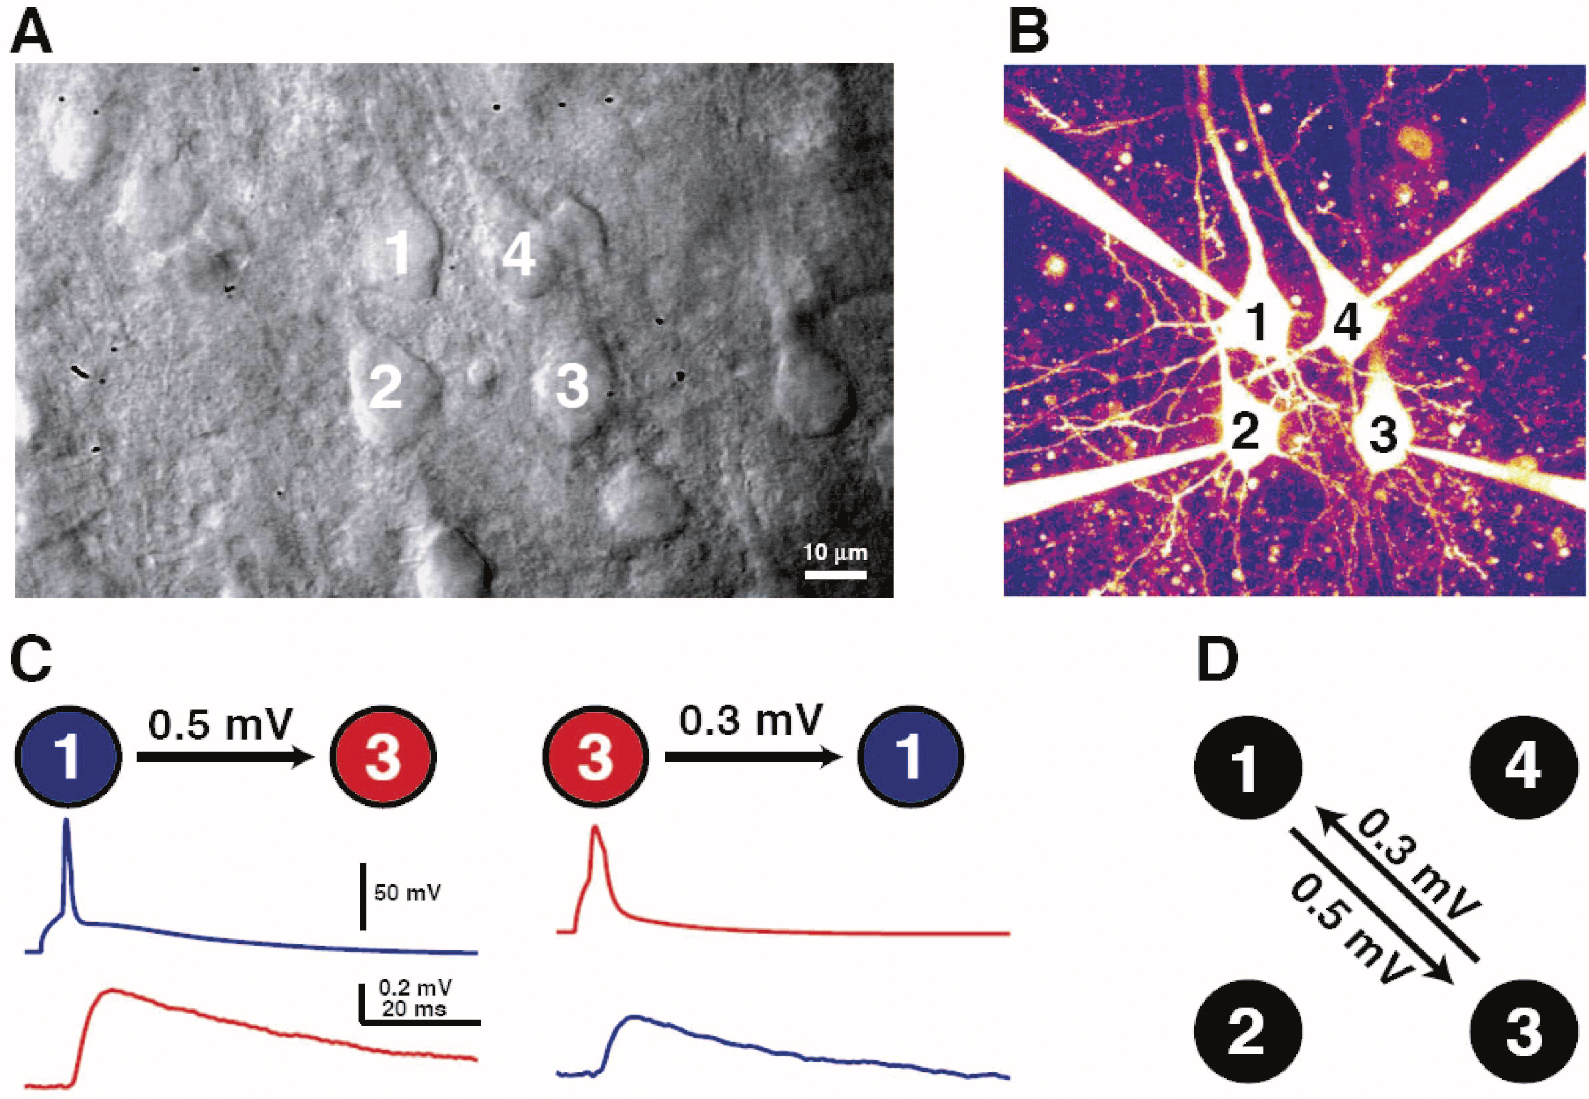
\includegraphics[width=.75\linewidth]{img/song2005-quadruplet_recordings.png}
  \caption{Song et al. use quadruple whole-cell recordings, observing
    simultaneously the membrane potential of four neurons.
    \textbf{A)} Contrast image showing four thick-tufted L5 neurons
    \textbf{B)} Fluorescent image of the same cells after patching on
    \textbf{C)} Evoking an action potential in the presynaptic neuron
    causes characteristic membrane potential change in the
    postsynaptic neuron \textbf{D)} Infering synaptic connectivity
    from the EPSP waveform observed in C). Image from \textcite{Song2005}.
    % \texttt{\textcolor{linkgrey}{3b056efe-3ebc}}
  }
\end{figure}
%\vspace{0.45cm}

While techniques for paired intracellular recordings are rapidly
developing, their ability to capture connectivity patterns of large
networks is yet very limited. To this date, the connectome of
\textit{C. Elegans} remains the outstanding exception of a
connectivity configuration that has been fully mapped
\parencite{White1986}. Even in the state-of-the-art experiment
conducted by Perin et al., using a setup capable of recording up to
twelve neurons simultaneously, the authors note that an investigation
of degree distribution was not carried out, due to lack of sufficient
data
\parencite{Perin2011}.

Working with a geometrical network model and its computational
\marginpar{exploiting the benefits of a geometrical model}
implementation, such restrictions disappear; the full information
about the network, in form of its connectivity matrix, is given at
point in time and can be easily queried for. Experiments that may take
days to perform \textit{in vivo}, can be completed in a matter of
seconds \textit{in silico}. As such, geometrical models lend
themselves to extensive examination of their structural aspects.  In
trying to exploit these advantages, two approaches present
themselves. One may construct a network model that extrapolates the
known biological configuration; a full structural examination of these
networks could possibly expose relevant patterns not yet observed. For
this approach a sophisticated understanding of the biological
configuration is critical. Neuron morphology, however, is difficult to
describe and extract. For this analysis we suggest a reductionist
approach. Having motivated an abstract model reflecting a cortical
network's anisotropy in connectivity, we distinguish emerging
structural patterns, specific to anisotropic networks, from results,
that only indirectly stem from the network's anisotropy, in the hopes
to be able to characterize the significance of directional
heterogeneity in structural connectivity of cortical circuits.


In this chapter we subject the anisotropic network model introduced in
Section~\ref{sec:anisotropic_network_model} to a critical analysis of
its structural aspects. General network topology, as well as specific
modes and patterns of connectivity, are to be identified and laid out
for comparison with findings in biological neural networks.  In an
effort to identify structural features that can be directly associated
with the network's anisotropy in connectivity, \marginpar{rewired and
  \mbox{distance-depen}\-dent networks as reference} it is crucial to
differentiate such findings from results that are only indirectly
caused by the network's anisotropy. To this end we are recruiting the
different network types introduced in the previous chapter throughout
this analysis. Having shown a decreasing degree of anisotropy in
rewired and distance-dependent networks, both models will serve as
reference to compare against for structural features found in
anisotropic networks. Analyzing standard graph measures in the first
two sections, we quickly move on to towards neuronal network specific
connectivity and anisotropy's role in being able to model such highly
non-random patterns in the later sections.


% ######################################################################### %
% ------------------------------------------------------------------------- %
%                             Comment Stuff
% ------------------------------------------------------------------------- %
% ######################################################################### %


% Human Connectome Project and the Open Connectome Project, the
% continued development of experimental techniques and of resources
% like the Brain Connectivity Toolbox software, as well as the
% research of theoreticians and experimentalists, are all dedicated
% towards the common goal of charting brain connectivity.

% In this general sense, brain connectivity can refer to linking
% between distinct units at various scales. From the mapping of fiber
% pathways between brain regions on the macroscale, to the synaptic
% connections of individual neurons on the microscale,
% [\textcolor{linkgrey}{Scholarpedia}].

% It is interesting not only to investigate for anatomical
% connections, but functional and causal as well. However, exploring
% the aspects of our specific geometric network model, in this chapter
% the connectivity of interest to us is the structural connectivity at
% the microscale, that is synaptic connections between individual
% neurons.

% \marginpar{Human Connectome Project
% \mbox{\url{humanconnectome.org}}}

% \parbox{1.8cm}{Human Connectome
% Project}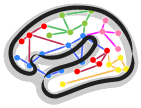
\includegraphics[width=0.45\linewidth]{img/HCP_logo.png}
% \mbox{\url{humanconnectome.org}}}


% Ho Ko connectivity -> specific dynamics.
% Pernice -> Spike Train Correlations. Maybe Shepherd 2005?

% ...and have been linked to brain function and dynamics.

% *What cool things synaptic connectivity does.  , stores memory, drives
% dynamics, etc.  While brain is plastic, there is structure that is
% believed to provide a framework, boundary conditions to

% *patterns of synaptic connectivity is neither completely random nor
% exclusively specific, patterns emerge [Sporns, Perin, Song]
 
% This specific, non-random connectivity largely impact dynamics and
% brain function:


% Connectivity in the directionally heterogenous geometric networks
% introduced in ??, models synaptic contacts between axon and
% dendrites of individual neurons. In this chapter

% It is then the task of this theoretical framework to provide results
% interesting to the biological situation. An investigation on how well
% an introduced model can reproduce certain structural aspects of
% networks that have already been fund is integral to the study of a
% computational model. But, furthermore, a model should aspire to
% extrapolate results found in the biological
% situation.



%%% Local Variables: 
%%% mode: latex
%%% TeX-master: "../dplths_document"
%%% End: 

% 
% ######################################################################### %
% ------------------------------------------------------------------------- %
%                     Degree distribution
% ------------------------------------------------------------------------- %
% ######################################################################### %

\section{Degree Distribution}\label{sec:degree_distribution}


The in- and out-degree of a vertex in a directed graph describes the
number of incoming and outgoing connection from and to other
\marginpar{cf. Definition~\ref{def:in_out_degree}} vertices. As a
fundamental concept in graph and network theory, the degree
distribution is integral in the categorization of networks and allows
for the estimation of graph properties. 

Node degree distribution was shown to have strong impact on the
dynamics of neuronal networks models commonly used in computational
neuroscience research \parencite{Roxin2011, Pernice2013}. Increasing
in-degree variance for example could be connected to the appearance of
oscillations in the network. Extracting degree distributions from
biological networks however, remains a challenge as many neurons need
to be tracked simultaneously to obtain enough data to confidently
estimate degree distributions.

\begin{figure}[H]
  \centering
  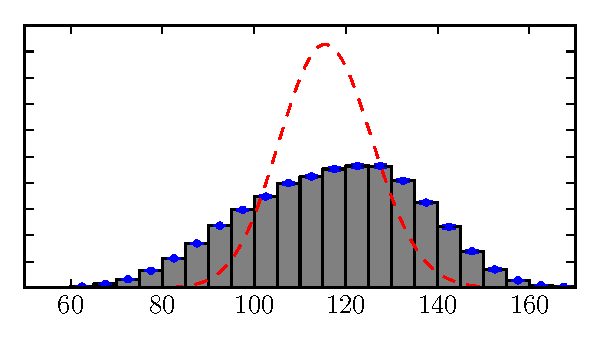
\includegraphics[width=0.65\textwidth]{%
    plots/9326138e.pdf}
  \caption{\textbf{In-degree distribution in anisotropic networks
      shows comparably high variance and is skewed to the left} From 250
    anisotropic networks in-degree distributions were extracted and
    are shown in a normed histogram plot, errorbars SEM. Comparison with the
    binomial degree distribution (red) of a Gilbert random graph model
    with matching parameter set ($N=1000$, $p =0.116$) shows higher
    variance of in-degrees in anisotropic networks (sample variance $=
    344.54$, variance of binomial distribution $Np(1-p) = 102.44$.)
    Skewness to the left of the sample is $-0.1763.$
    (\smtcite{9326138e})}
  \label{fig:in_degree_ER_compare}
\end{figure}

Here we analyze in- and out-degrees in the anisotropic network
model. First we find that compared to the binomial in-degree
distribution of a Gilbert random graph model, in-degrees of vertices
in anisotropic networks display higher variance and their distribution
is skewed to the left (\autoref{fig:in_degree_ER_compare}). However,
this specific in-degree profile is not an intrinsic property of
anisotropy, as the distribution remains stable under manipulation of
the anisotropy degree and closely matches the profile of a purely
distance-dependent network (\autoref{fig:in_degree_rewiring}). This
result agrees with findings of \textcite[Fig. S3]{Perin2011}, who were
able to recreate degree distributions from their experiment with layer
5 thick-tufted pyramidal cells in neonatal rats from the extracted
distance-dependent connection profiles alone.

\begin{figure}[H]
  \centering
  \renewcommand{\tabcolsep}{2pt}
  \setlength\extrarowheight{0pt}
  \begin{tabular}{lll}
    \begin{overpic}[width=0.28\textwidth]{%
        plots/77995b6b_in000.pdf}
      \put(12,56){\small $\eta = 0$}
    \end{overpic}
    &
    \begin{overpic}[width=0.28\textwidth]{%
        plots/77995b6b_in025.pdf}
      \put(12,56){\small $\eta = 0.25$}
    \end{overpic}
    &
    \begin{overpic}[width=0.28\textwidth]{%
        plots/77995b6b_in050.pdf}
      \put(12,56){\small $\eta = 0.5$}
    \end{overpic}
    \\
    \begin{overpic}[width=0.28\textwidth]{%
        plots/77995b6b_in075.pdf}
      \put(12,56){\small $\eta = 0.75$}
      \put(4,-4){\small$0$}\put(78,-4){\small$200$}
    \end{overpic}
    &
    \begin{overpic}[width=0.28\textwidth]{%
        plots/77995b6b_in100.pdf}
      \put(12,56){\small $\eta = 1$}
      \put(4,-4){\small$0$}\put(78,-4){\small$200$}
    \end{overpic}
    & 
    \begin{overpic}[width=0.28\textwidth]{%
        plots/77995b6b_indst.pdf}
      \put(12,56){\small distance}
      \put(4,-4){\small$0$}\put(78,-4){\small$200$}
    \end{overpic}
    \\
  \end{tabular}
  \caption{\textbf{In-degree distribution not affected by varying
      degrees of anisotropy} In-degree distributions from the 25
    sample graphs and their rewiring stages are plotted in normed
    histograms and listed from rewiring factor $\eta =0$ (original
    anisotropic) to $\eta = 1$ (completely rewired, maximal
    isotropy). Comparison shows that varying degrees of anisotropy do
    not influence the degree distribution, in fact in-degree
    distributions match with the degree distribution of an equivalent
    distance-dependent network shown bottom-right
    (\smtcite{77995b6b}). }
  \label{fig:in_degree_rewiring}
\end{figure}


While the out-degree distribution of vertices in the anisotropic
network also shows itself stable under rewiring, its distribution is
drastically different from the out-degree distribution in a comparable
distance-dependent network (\autoref{fig:out_degree_rewiring}). The
asymmetric, long-tailed distribution is identified as an artifact of
the anisotropic network's spatial confinement; a neuron, closely
located near a surface edge, might have an axon projection out of the
square causing minimal out-degree or, projecting through the entire
length of the surface, may have maximal out-degree. Approximating the
expected number of outgoing connections for a vertex in an anisotropic
network of size $N$, side-length $s$ and axon width $w$ as
\[
  N \frac{w l}{s^2},
\]
with parameters $N = 1000$ and $\frac{w}{s} = 0.252$, we obtain an
upper bound for the expected out-degree, 
\[
  N \frac{w l}{s^2} \leq N\frac{w}{s} \sqrt{2} \approx 350.
\]
If $f(l)$ is the probability density function to find axon length $l$
for a random node $v$ in the anisotropic network model, the out-degree
distribution is then approximated by
%
\begin{align}\label{eq:axon_length_approx}
  \mathbf{P}(d_{\mathrm{out}}(v) = N \frac{w l}{s^2}) = f(l),  
\end{align}
%
see also \autoref{fig:out_degree_ER_compare}.

\begin{figure}[H]
  \centering
  \renewcommand{\tabcolsep}{2pt}
  \setlength\extrarowheight{0pt}
  \begin{tabular}{lll}
    \begin{overpic}[width=0.28\textwidth]{%
        plots/77995b6b_out000.pdf}
      \put(12,56){\small $\eta = 0$}
    \end{overpic}
    &
    \begin{overpic}[width=0.28\textwidth]{%
        plots/77995b6b_out025.pdf}
      \put(12,56){\small $\eta = 0.25$}
    \end{overpic}
    &
    \begin{overpic}[width=0.28\textwidth]{%
        plots/77995b6b_out050.pdf}
      \put(12,56){\small $\eta = 0.5$}
    \end{overpic}
    \\
    \begin{overpic}[width=0.28\textwidth]{%
        plots/77995b6b_out075.pdf}
      \put(12,56){\small $\eta = 0.75$}
      \put(4,-4){\small$0$}\put(78,-4){\small$350$}
    \end{overpic}
    &
    \begin{overpic}[width=0.28\textwidth]{%
        plots/77995b6b_out100.pdf}
      \put(12,56){\small $\eta = 1$}
      \put(4,-4){\small$0$}\put(78,-4){\small$350$}
    \end{overpic}
    & 
    \begin{overpic}[width=0.28\textwidth]{%
        plots/77995b6b_outdst.pdf}
      \put(52,56){\small distance}
      \put(4,-4){\small$0$}\put(78,-4){\small$350$}
    \end{overpic}
    \\
  \end{tabular}
  \caption{\textbf{Out-degree distribution not affected by varying
      anisotropy but highly different from distance-dependent
      networks} Out-degree distributions from the 25 sample graphs and
    their rewiring stages are plotted in normed histograms and listed
    from rewiring factor $\eta =0$ (original anisotropic) to $\eta =
    1$ (completely rewired, maximal isotropy). While varying degrees
    of anisotropy do not influence the degree distribution, the
    characteristic out-degree profile is drastically different from
    the distribution found in equivalent distance-dependent networks
    (\smtcite{77995b6b}). }
  \label{fig:out_degree_rewiring}
\end{figure}


%------------------------------------------------
\marginpar{\vspace{1.91cm}\\Steep incline for small out-degree cut off
  due to binning (cf. \autoref{suppfig:out_degree})} 
%------------------------------------------------
\begin{figure}[H]
  \centering
  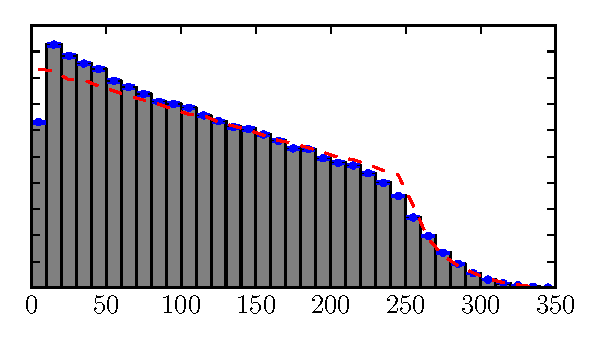
\includegraphics[width=0.65\textwidth]{%
    plots/019555b0.pdf}
  \caption{\textbf{Characteristic out-degree distribution as an
      artifact of network's boundaries} From 250 anisotropic networks
    out-degree distributions were extracted and are shown in a normed
    histogram plot, errorbars SEM. The characteristic distribution is
    identified as an artifact of the network's spatial confinement;
    using equation~\ref{eq:axon_length_approx} the out-degree profile
    is approximated (red) by the distribution of axon lengths in the
    anisotropic network (\smtcite{019555b0}).}
  \label{fig:out_degree_ER_compare}
\end{figure}



%%% Local Variables: 
%%% mode: latex
%%% TeX-master: "../dplths_document"
%%% End: 

 
% ######################################################################### %
% ------------------------------------------------------------------------- %
%                        Small World Properties
% ------------------------------------------------------------------------- %
% ######################################################################### %


\section{Small World Properties}\label{sec:small_world}

Sporns papers


%%% Local Variables: 
%%% mode: latex
%%% TeX-master: "../dplths_document"
%%% End: 

 
\section{Two Neuron Connections}

Connectivity in cortical neural networks shows a specific . First
described by Markram 1997, finding across have confirmed . 

A first result


\begin{figure}[htp]
  \centering
  \makebox{%
    \begin{overpic}[height=0.17\textheight]{%
        plots/c5f1462b_aniso_rand.pdf}
      %\put(89.8,56.5){\small\textbf{A}}
      %\put(14.3,78.9){\small\textbf{A}}
    \end{overpic}
    \hspace{0.45cm}
    \begin{overpic}[height=0.17\textheight]{%
        plots/c5f1462b_aniso_rew.pdf}      
       %\put(16.2,78.9){\small\textbf{B}}
      %\put(12,5){\small\textbf{B}}
    \end{overpic}
  }%
  \vspace{0.2cm}
  \caption{\textbf{Title} SEM!  (\smtcite{c5f1462b}).} %?? fix width issue!!
  \label{fig:two_neuron_probs}
\end{figure}  


%%% Local Variables: 
%%% mode: latex
%%% TeX-master: "../dplths_document"
%%% End: 

% 

\section{Motifs}

In this chapter we analyze the strucarl. The term motif referes
to... . Studies of \textcite{Song2005} and \textcite{Perin2011} show
stuff.

\subsection*{Three-neuron patterns}

Song motifs:


\begin{figure}[H]
  \centering
  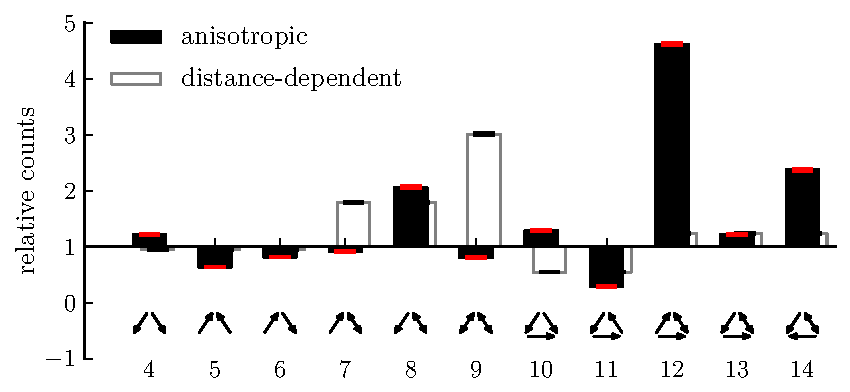
\includegraphics[width=0.95\linewidth]{%
    plots/4839ce41_aniso_dist.pdf} 
  \captionsetup{skip=8pt}
  \caption{\textbf{Relative occurrence of three-neuron patterns}
    Extracting the counts of three-node motifs in anisotropic (filled
    bars) and distance-dependent networks (unfilled bars), the
    quotient of the obtained count with the number of occurrences
    expected from the two-neuron connection probabilities in the
    networks (rs =, ,, cf.) shows the over- and underrepresentation of
    specific motifs in the network (red and black errorbars are
    SEM). In anisotropic networks pattern number \enquote{12}, for
    example, appears around five times more often than we would expect
    from the occurrence two-neuron connections. The relative counts
    for anisotropic networks resemble the findings of
    \textcite{Song2005} and differ significantly from the counts in
    distance-dependent networks, implying that anisotropy has a strong
    influence on the relative occurrence of three-neuron
    patterns. (\smtcite{4839ce41}) }
  \label{fig:distance_theory_compare}
\end{figure}




\begin{figure}[H]
  \centering
  \includegraphics[width=0.95\linewidth]{%
    plots/7c826e10_test.pdf} 
  \captionsetup{skip=8pt}
  \caption{\textbf{Relative occurrence of three-neuron patterns}
    Extracting the counts of three-node motifs in anisotropic (filled
    bars) and distance-adependent networks (unfilled bars), the
    quotient of the obtained count with the number of occurrences
    expected from the two-neuron onnection probabilities in the
    networks (rs =, ,, cfsdfg.) shows the over- and underrepresentation of
    specific motifs in the network (red and black errorbars are
    SEM). In anisotropic networks pattern number \enquote{12}, for
    example, appears around five times more often than we would expect
    from the occurrele the findings of
    \textcite{Song2005} and differ significantly from the counts in
    distance-dependent networks, implying that anisotropy has a strong
    influence on the relative occurrence of three-neuron
    patterns. (\smtcite{4839ce41}) }
  \label{fig:distance_theory_compare}
\end{figure}



\begin{figure}[H]
  \centering
  \renewcommand{\tabcolsep}{0pt}
  \setlength\extrarowheight{0pt}
  \begin{tabular}{ll}
    \begin{overpic}[width=0.5\textwidth]{%
        /users/hoffmann/research/cn_k_test.pdf}
      %\put(12,56){\small $\eta = 0$}
    \end{overpic}
    &
    \begin{overpic}[width=0.5\textwidth]{%
        /users/hoffmann/research/cn_k_test.pdf}
      %\put(12,56){\small $\eta = 0.25$}
    \end{overpic}
    \\
    \begin{overpic}[width=0.5\textwidth]{%
        /users/hoffmann/research/cn_k_test.pdf}
      %\put(12,56){\small $\eta = 0.5$}
    \end{overpic}
    &
    \begin{overpic}[width=0.5\textwidth]{%
        /users/hoffmann/research/cn_k_test.pdf}
      % \put(12,56){\small $\eta = 0.75$}
      %\put(4,-4){\small$0$}\put(78,-4){\small$200$}
    \end{overpic}
    \\
    % \begin{overpic}[width=0.28\textwidth]{%
    %     plots/77995b6b_in100.pdf}
    %   \put(12,56){\small $\eta = 1$}
    %   \put(4,-4){\small$0$}\put(78,-4){\small$200$}
    % \end{overpic}
    % & 
    % \begin{overpic}[width=0.28\textwidth]{%
    %     plots/77995b6b_indst.pdf}
    %   \put(12,56){\small distance}
    %   \put(4,-4){\small$0$}\put(78,-4){\small$200$}
    % \end{overpic}
    % \\
  \end{tabular}
  \caption{\textbf{In-degxree distrbution not affected by varying
      degrees of anisotropy} 
    (\smtcite{77995b6b}). }
  \label{fig:in_degree_rewiring}
\end{figure}



%%% Local Variables: 
%%% mode: latex
%%% TeX-master: "../dplths_document"
%%% End: 

















%%% Local Variables: 
%%% mode: latex
%%% TeX-master: "../dplths_document"
%%% End: 


%% ************************************************
\chapter{Test Chapter}\label{ch:test_chapter} 
% ************************************************

\begin{pythoncode} %underscore problem!!
data_paths = sys.argv[1:1+params.n_data_sets]
data_sets = []

for data_path in data_paths:
    pfile = open(data_path, "rb")
    data_sets.append(pickle.load(pfile))
    pfile.close()

try:
    sys.argv[1+params.n_data_sets]
except IndexError:
    label = img_label.labelstr
else:
    label = sys.argv[1+params.n_data_sets]
\end{pythoncode}




%%% Local Variables: 
%%% mode: latex
%%% TeX-master: "../dplths_document"
%%% End: 




%\include{multiToC} % <--- just debug stuff, ignore for your documents

% ********************************************************************
% Backmatter
%*******************************************************

% \appendix
% \cleardoublepage
% \part{Appendix}
% %*******************************************************
% Appendix
%*******************************************************
% If problems with the headers: get headings in appendix etc. right
%\markboth{\spacedlowsmallcaps{Appendix}}{\spacedlowsmallcaps{Appendix}}

\chapter{Appenidx}

\section{Mathematica}

% \newgeometry{left=1.0in,right=1.0in}

\begin{mathematica}[ht!]
  \centering
  \captionsetup{format=plain, font=normal}
  \includegraphics[width=\linewidth, cframe=RoyalBlue 1pt]{mathematica/distance_theorem.pdf}
  \caption{Computation of probability density function for distance
    between to random points in square of side length $s$ as supplement
    to proof of Theorem~\ref{theorem:distance_square}. Note that form of
    final result \texttt{Out[7]} differs from solution given in
    \ref{theorem:distance_square}. While proof of equivalence could not
    be achieved analytically, expressions given are numerically
    equivalent, see \autoref{mathematica:comparison}.}
  \label{mathematica:distances}
\end{mathematica} 


\begin{mathematica}[t]
  \centering
  \captionsetup{format=plain, font=normal}
  \includegraphics[width=\linewidth, cframe=RoyalBlue 1pt]{%
    mathematica/distance_theorem.pdf}
  \caption{Computation of probability density function for distance
    between to random points in square of side length $s$ as supplement
    to proof of Theorem~\ref{theorem:distance_square}. Note that form of
    final result \texttt{Out[7]} differs from solut}
  \label{mathematica:comparison}
\end{mathematica} 




% ######################################################################### %
% ------------------------------------------------------------------------- %
%                 Reproducibility in Computational Research         
% ------------------------------------------------------------------------- %
% ######################################################################### %

%\section{Reproducibility in Computational Research}\label{sec:reproducibility}

%\textcite{Sumatra2012}




% ######################################################################### %
% ------------------------------------------------------------------------- %
%                         Supplementary Figures
% ------------------------------------------------------------------------- %
% ######################################################################### %

\section{Supplementary figures}\label{sec:supp_figures}

\subsection*{\autoref{ch:network_model}}

\begin{figure}[H]
  \centering
  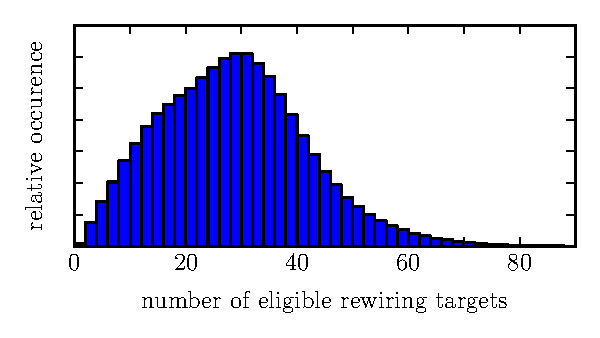
\includegraphics[width=0.8\textwidth]{%
    plots/4afc2727.pdf}
  \caption{(\smtcite{4afc2727})}
  \label{suppfig:rew_stats}
\end{figure}


\subsection*{\autoref{ch:structural_aspects}}

\begin{figure}[H]
  \centering
  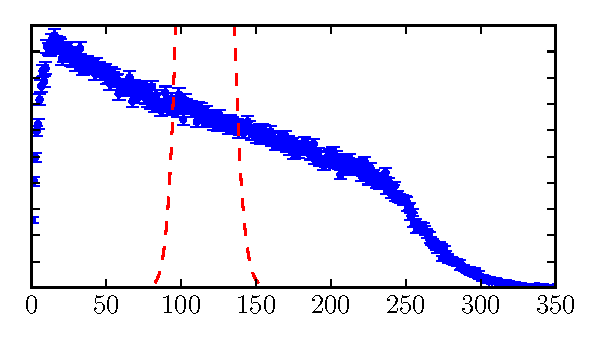
\includegraphics[width=0.7\textwidth]{%
    plots/c7ee86d7.pdf}
  \caption{(\smtcite{c7ee86d7})}
  \label{suppfig:out_degree}
\end{figure}


\begin{figure}[htp]
  \centering
  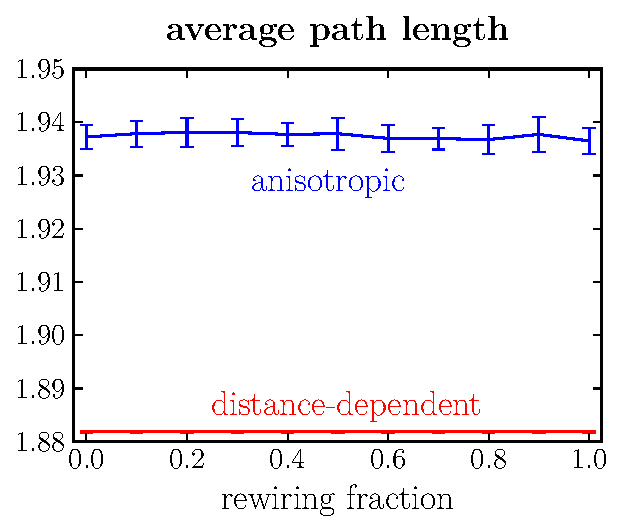
\includegraphics[width=0.5\textwidth]{plots/064f9b10_apl_1000.pdf}
  \caption{Average path length for anisotropic and distance-dependent
    networks, $N=1000$. (\smtcite{064f9b10})} %?? fix width issue!!
  \label{suppfig:small_world}
\end{figure}


\begin{figure}[htp]
  \centering
  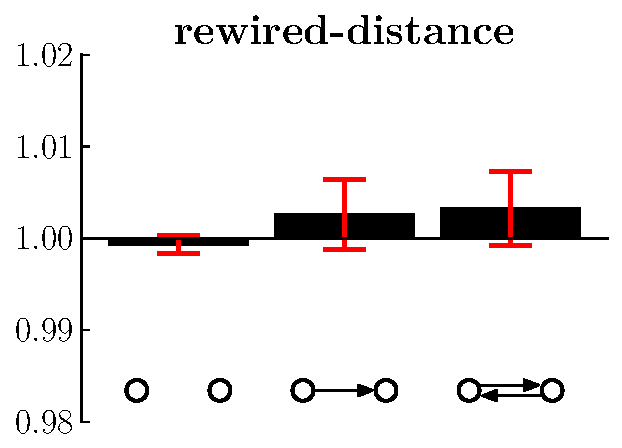
\includegraphics[width=0.5\textwidth]{plots/c5f1462b_rew_dist.pdf}
  \caption{Probabilities for connections in neuron pairs are identical
    in distance-dependent and rewired anisotropic
    networks. (\smtcite{c5f1462b})} %?? fix width issue!!
  \label{suppfig:two_neurons_dist_rew}
  \end{figure}


\begin{figure}
    \renewcommand{\tabcolsep}{1pt}
    \setlength\extrarowheight{0pt}
    \begin{tabular}{lll}
      \begin{overpic}[width=0.33\textwidth]{%
          plots/5841710e_all_overall}
        %\put(12,55){\small $\eta = 0$}
      \end{overpic}
      &
      \begin{overpic}[width=0.33\textwidth]{%
          plots/5841710e_all_single.pdf}
        %\put(12,55){\small $\eta = 0.25$}
      \end{overpic}
      &
      \begin{overpic}[width=0.33\textwidth]{%
          plots/5841710e_all_recip.pdf}
        %\put(12,55){\small $\eta = 0.33$}
      \end{overpic}
      \\
      \begin{overpic}[width=0.33\textwidth]{%
          plots/5841710e_in_overall.pdf}
        %\put(12,55){\small $\eta = 0.75$}
      \end{overpic}
      &
      \begin{overpic}[width=0.33\textwidth]{%
          plots/5841710e_in_single.pdf}
        %\put(12,55){\small $\eta = 1$}
        %\put(4,-4){$0$}%\put(78,-4){$200$}
      \end{overpic}
      & 
      \begin{overpic}[width=0.33\textwidth]{%
          plots/5841710e_in_recip.pdf}
        %\put(12,55){\small distance}
        %\put(4,-4){$0$}%\put(78,-4){$200$}
      \end{overpic}
      \\
      \begin{overpic}[width=0.33\textwidth]{%
          plots/5841710e_out_overall.pdf}
        %\put(12,55){\small $\eta = 0.75$}
      \end{overpic}
      &
      \begin{overpic}[width=0.33\textwidth]{%
          plots/5841710e_out_single.pdf}
        %\put(12,55){\small $\eta = 1$}
        %\put(4,-4){$0$}%\put(78,-4){$200$}
      \end{overpic}
      & 
      \begin{overpic}[width=0.33\textwidth]{%
          plots/5841710e_out_recip.pdf}
        %\put(12,55){\small distance}
        %\put(4,-4){$0$}%\put(78,-4){$200$}
      \end{overpic}
    \end{tabular}
  \caption{Common neighbor rule for overall connection probability,
    single connections and reciprocal connections in anisotropic
    (blue), rewired (red), distance-dependent (green) and tuned
    anisotropic (orange) networks. (\smtcite{5841710e})} 
  \label{suppfig:common_neighbor}
  \end{figure}

% \begin{figure}[H]
%   \centering
%   \includegraphics{

%%% Direct in Chapter.

% \begin{minipage}[t]{0.48\textwidth}
% \begin{align*}
% % \mathbf{P}(X=1) &    =   p_u^3  \\
% % \mathbf{P}(X=2) &    =   6 p_u p_u p_s\\
% % \mathbf{P}(X=3) &    =   3 p_u p_u p_r\\
% \mathbf{P}(X=4) &    =   3 p_s^2 p_u\\
% \mathbf{P}(X=5) &    =   3 p_s^2 p_u\\
% \mathbf{P}(X=6) &    =   6 p_s^2 p_u\\
% \mathbf{P}(X=7) &    =   6 p_s p_u p_r\\
% \mathbf{P}(X=8) &    =   6 p_s p_u p_r\\
% \mathbf{P}(X=9) &    =   3 p_r^2 p_u\\
% \end{align*}
% \end{minipage}%
% \begin{minipage}[t]{0.48\textwidth}
% \begin{equation}
% \label{eq:three_motif_full}
% \begin{aligned}
% \mathbf{P}(X=10) &   =   6 p_s^3   \\
% \mathbf{P}(X=11) &   =   2 p_s^3    \\
% \mathbf{P}(X=12) &   =   3 p_s^2 p_r\\
% \mathbf{P}(X=13) &   =   6 p_s^2 p_r\\
% \mathbf{P}(X=14) &   =   3 p_s^2 p_r\\
% \mathbf{P}(X=15) &   =   6 p_s p_r^2\\
% \mathbf{P}(X=16) &   =   p_r^3 
% \end{aligned}
% \end{equation}
% \end{minipage}


%%% Local Variables: 
%%% mode: latex
%%% TeX-master: "../dplths_document"
%%% End: 

%********************************************************************
% Other Stuff in the Back
%*******************************************************
\cleardoublepage%********************************************************************
% Bibliography
%*******************************************************
% work-around to have small caps also here in the headline


% \manualmark
% \markboth{\spacedlowsmallcaps{\bibname}}{\spacedlowsmallcaps{\bibname}} % work-around to have small caps also
% %\phantomsection 
% \refstepcounter{dummy}
% \addtocontents{toc}{\protect\vspace{\beforebibskip}} % to have the bib a bit from the rest in the toc
% \addcontentsline{toc}{chapter}{\tocEntry{\bibname}}
% \bibliographystyle{plainnat}
% \label{app:bibliography} 
% \bibliography{Bibliography}


\printbibliography

%%% Local Variables: 
%%% mode: latex
%%% TeX-master: "../dplths_document"
%%% End: 

% \cleardoublepage\pagestyle{empty}

\hfill

\vfill


\pdfbookmark[0]{Colophon}{colophon}
\section*{Colophon}
This document was typeset using the typographical look-and-feel \texttt{classicthesis} developed by Andr\'e Miede. 
The style was inspired by Robert Bringhurst's seminal book on typography ``\emph{The Elements of Typographic Style}''. 
\texttt{classicthesis} is available for both \LaTeX\ and \mLyX: 
\begin{center}
\url{http://code.google.com/p/classicthesis/}
\end{center}
Happy users of \texttt{classicthesis} usually send a real postcard to the author, a collection of postcards received so far is featured here: 
\begin{center}
\url{http://postcards.miede.de/}
\end{center}
 
\bigskip

\noindent\finalVersionString

%Hermann Zapf's \emph{Palatino} and \emph{Euler} type faces (Type~1 PostScript fonts \emph{URW
%Palladio L} and \emph{FPL}) are used. The ``typewriter'' text is typeset in \emph{Bera Mono}, 
%originally developed by Bitstream, Inc. as ``Bitstream Vera''. (Type~1 PostScript fonts were made 
%available by Malte Rosenau and
%Ulrich Dirr.)

%\paragraph{note:} The custom size of the textblock was calculated
%using the directions given by Mr. Bringhurst (pages 26--29 and
%175/176). 10~pt Palatino needs  133.21~pt for the string
%``abcdefghijklmnopqrstuvwxyz''. This yields a good line length between
%24--26~pc (288--312~pt). Using a ``\emph{double square textblock}''
%with a 1:2 ratio this results in a textblock of 312:624~pt (which
%includes the headline in this design). A good alternative would be the
%``\emph{golden section textblock}'' with a ratio of 1:1.62, here
%312:505.44~pt. For comparison, \texttt{DIV9} of the \texttt{typearea}
%package results in a line length of 389~pt (32.4~pc), which is by far
%too long. However, this information will only be of interest for
%hardcore pseudo-typographers like me.%
%
%To make your own calculations, use the following commands and look up
%the corresponding lengths in the book:
%\begin{verbatim}
%    \settowidth{\abcd}{abcdefghijklmnopqrstuvwxyz}
%    \the\abcd\ % prints the value of the length
%\end{verbatim}
%Please see the file \texttt{classicthesis.sty} for some precalculated 
%values for Palatino and Minion.
%
%    \settowidth{\abcd}{abcdefghijklmnopqrstuvwxyz}
%    \the\abcd\ % prints the value of the length





% \cleardoublepage%*******************************************************
% Declaration
%*******************************************************
\refstepcounter{dummy}
\pdfbookmark[0]{Declaration}{declaration}
\chapter*{Erklärung}
\thispagestyle{empty}
Put your declaration here.
\bigskip
 
\noindent\textit{\myLocation, \myTime}

\smallskip

\begin{flushright}
    \begin{tabular}{m{5cm}}
        \\ \hline
        \centering\myName \\
    \end{tabular}
\end{flushright}

% ********************************************************************
% Game Over: Restore, Restart, or Quit?
%*******************************************************


% %********************************************************************
% Index
%*******************************************************
% work-around to have small caps also here in the headline


\manualmark
\markboth{\spacedlowsmallcaps{\bibname}}{\spacedlowsmallcaps{\bibname}} % work-around to have small caps also
%\phantomsection 
\refstepcounter{dummy}
\addtocontents{toc}{\protect\vspace{\beforebibskip}} % to have the bib a bit from the rest in the toc
\addcontentsline{toc}{chapter}{\tocEntry{Index}}
% \bibliographystyle{plainnat}
% \label{app:bibliography} 
% \bibliography{Bibliography}


\printindex


%%% Local Variables: 
%%% mode: latex
%%% TeX-master: "../dplths_document"
%%% End: 

% 
%*******************************************************
% List of Symbols
%*******************************************************
% work-around to have small caps also here in the headline


% \manualmark
% \markboth{\spacedlowsmallcaps{\bibname}}{\spacedlowsmallcaps{\bibname}} % work-around to have small caps also
% %\phantomsection 
% \refstepcounter{dummy}
% \addtocontents{toc}{\protect\vspace{\beforebibskip}} % to have the bib a bit from the rest in the toc
% \addcontentsline{toc}{chapter}{\tocEntry{\bibname}}
% \bibliographystyle{plainnat}
% \label{app:bibliography} 
% \bibliography{Bibliography}

\begin{longtable}[l]{p{75pt} p{200pt}} 
\textbf{Symbol}	&  \textbf{Description} \\ 
$L$	& Length\\ 
$Ma$	& Mach number\\
 $p$	& Pressure 
%... 
\end{longtable}



%%% Local Variables: 
%%% mode: latex
%%% TeX-master: "../dplths_document"
%%% End: 



\end{document}
% ********************************************************************
